%!TEX program = xelatex
\PassOptionsToPackage{usenames,dvipsnames}{color}
\documentclass{beamer}
% 这里[]里可以有很多选项,为了打印讲演稿可以增加handout或者trans
%%%%%%%%%%%%%%%%%%%%%%%%%%%%%%%%%%%%%%%%%%%%%%%%%%%%%%%%%%%%%%%%%%%%%%%%%%%%%%%%%%%%%%%%%%%%%%%%%%%%%%%%%

%%%%%%%%%%%%%%%%%%%%%%%%%%%%%%%%%利用一些包%%%%%%%%%%%%%%%%%%%%%%%%%%%%%%%%%%%%%%%%%%%%%%%%%%%%%%%%%%%%%
\usepackage{xcolor}
\usepackage{amsmath,amssymb}%AMS系列宏包中最重要的,引进数学环境如{align}
\usepackage{amsfonts}%数学符号与字体
\usepackage{multicol}%正文双栏
\usepackage{bm}%数学符号黑斜体
\usepackage{graphicx}
\usepackage{subfigure}
\usepackage{multirow}%跨行表格
\usefonttheme[onlymath]{serif}%beamer中数学字体改为Euclid
%%%%%%%%%%%%%%%%%%%%%%%%%%%%%%%%%%%%%%%%%%%%%%%%%%%%%%%%%%%%%%%%%%%%%%%%%%%%%%%%%%%%%%%%%%%%%%%%%%%%%%%%%
%%%%%%%%%% 额外的
\usepackage{ragged2e}%文字两端对齐
\renewcommand{\raggedright}{\leftskip=0pt \rightskip=0pt plus 0cm}%文字两端对齐

\usepackage{setspace}	%change line space:\begin{spacing}{1.3}...\end{spacing}
%\space{1.5}{...}

\setbeamertemplate{caption}[numbered] %显示序号;beamer默认图表不加序号: https://yihui.name/cn/2010/08/show-caption-numbers-in-beamer/

\usepackage{caption}%不显示图表的caption中"Figure:"
\captionsetup[figure]{labelformat=empty}% redefines the caption setup of the figures environment in the beamer class.
%https://tex.stackexchange.com/questions/82456/how-to-remove-figure-caption-prefix-figure-in-beamer

\RequirePackage{natbib} %引用格式

% \usepackage{hyperref}
% \hypersetup{
%      colorlinks,
%      urlcolor    = blue
% }%https://tex.stackexchange.com/questions/401884/how-do-i-change-hyperlinks-color-only/401885

\usepackage{url}
%\def\UrlFont{\em}
\def\UrlFont{\sf}%等同于\urlstyle{tt}

\usepackage{tikz}
\usepackage{amsmath}
\usetikzlibrary{arrows,shapes}

\definecolor{DeepSkyBlue3}{RGB}{0,154,205}
\definecolor{DarkOrange}{RGB}{255,140,0}
\definecolor{HotPink}{RGB}{255,105,180}
\definecolor{DeepPink3}{RGB}{205 16 118}
\definecolor{DarkSlateBlue}{RGB}{72,61,139}
\definecolor{Indigo}{RGB}{75,0,130}
\definecolor{MidnightBlue}{RGB}{25,25,112}
\definecolor{BGpurple}{RGB}{185 181 205}

%%%%%%%%%%%%%%%%%%%%%%%%%%%%%%%%%%%%%%重定义字体、字号命令 %%%%%%%%%%%%%%%%%%%%%%%%%%%%%%%%%%%%%%%%%%%%%%
\newcommand{\sscd}{\fontspec{SverigeScriptCleanDemo.TTF}}
\newcommand{\scin}{\fontspec{SCRIPTIN.TTF}}
\newcommand{\grvi}{\fontspec{GreatVibes.OTF}}
\newcommand{\arab}{\fontspec{ArabellaDemo.TTF}}
%%%%%%%%%%%%%%%%%%%%%%%%%%%%%%%%%%%%%%%%%%%%%%%%%%%%%%%%%%%%%%%%%%%%%%%%%%%%%%%%%%%%%%%%%%%%%%%%%%%%%%%%

%%%%%%%%%%%%%%%%%%%%%%%%%%%%%%%%%%%%%%%设置主题%%%%%%%%%%%%%%%%%%%%%%%%%%%%%%%%%%%%%%%%%%%%%%%%%%%%%%%%%
\usetheme{Singapore}
% 这里还可以选择别的主题Bergen,Boadilla,Madrid,AnnArbor,CambridgeUS,Pittsburgh
% Rochester. 有导航栏的Antibes,JuanLesPins,Montpellier,有内容的Berkeley,PaloAlto,
% Goettingen,Marburg,Hannover,有最小导航栏的Berlin,Ilmenau,Dresden,Darmstadt,
% Frankfurt,Singapore,Szeged,有章和节表单的Copenhagen,Luebeck,Malmoe,Warsaw
%%%%%%%%%%%%%%%%%%%%%%%%%%%%%%%%%%%%%%%%%%%%%%%%%%%%%%%%%%%%%%%%%%%%%%%%%%%%%%%%%%%%%%%%%%%%%%%%%%%%%%%%

%%%%%%%%%%%%%%%%%%%%%%%%%%%%%%%%%%%%%%%设置颜色主题%%%%%%%%%%%%%%%%%%%%%%%%%%%%%%%%%%%%%%%%%%%%%%%%%%%%%
\usecolortheme{crane}
% 这个主题一般选择动物来命名
% 这里还可以选择别的颜色主题,如默认的和有特别目的的颜色主题default,structure,sidebartab,全颜色主题albatross,
% beetle,crane,dove,fly,seagull,wolverine,beaver
%%%%%%%%%%%%%%%%%%%%%%%%%%%%%%%%%%%%%%%%%%%%%%%%%%%%%%%%%%%%%%%%%%%%%%%%%%%%%%%%%%%%%%%%%%%%%%%%%%%%%%%%

%%%%%%%%%%%%%%%%%%%%%%%设置内部颜色主题(这些主题一般改变block里的颜色)%%%%%%%%%%%%%%%%%%%%%%%%%%%%%%%%%%
\usecolortheme{lily}
% 这个主题一般选择植物来命名
% 这里还可以选择别的颜色主题,如默认的和有特别目的的颜色主题lily,orchid,rose,crane
%%%%%%%%%%%%%%%%%%%%%%%%%%%%%%%%%%%%%%%%%%%%%%%%%%%%%%%%%%%%%%%%%%%%%%%%%%%%%%%%%%%%%%%%%%%%%%%%%%%%%%%%

%%%%%%%%%%%%%%%%%%%%%%%设置外部颜色主题(这些主题一般改变title里的颜色)%%%%%%%%%%%%%%%%%%%%%%%%%%%%%%%%%%
\usecolortheme{dolphin}
% 这个主题一般选择海洋动物来命名
% 这里还可以选择别的颜色主题,如默认的和有特别目的的颜色主题whale,seahorse,dolphin
%%%%%%%%%%%%%%%%%%%%%%%%%%%%%%%%%%%%%%%%%%%%%%%%%%%%%%%%%%%%%%%%%%%%%%%%%%%%%%%%%%%%%%%%%%%%%%%%%%%%%%%%

%%%%%%%%%%%%%%%%%%%%%%%%%%%%%%%%%%%%%%%%%%%%设置字体主题%%%%%%%%%%%%%%%%%%%%%%%%%%%%%%%%%%%%%%%%%%%%%%%%
\usefonttheme{professionalfonts}
% 类似的还可以定义structurebold,structuresmallcapsserif,professionalfonts
%%%%%%%%%%%%%%%%%%%%%%%%%%%%%%%%%%%%%%%%%%%%%%%%%%%%%%%%%%%%%%%%%%%%%%%%%%%%%%%%%%%%%%%%%%%%%%%%%%%%%%%%
\begin{document}
%%%%%%%%%%%%%%%%%%%%%%%%%%%%%%%%%%%%%%%%%%%%%%%%%%%%%%%%%%%%%
{%BACKGROUND START
\usebackgroundtemplate{
\includegraphics[width=\paperwidth]{fig/BG.png}}
\title{Variational Auto-Encoder}    %标题
\subtitle{Explainations \& Experiments}   %副标题
\author{Tianwei Yue}  % 作者
\date{\today}   %日期
\frame{\titlepage}
}%BACKGROUND E N D
%%%%%%%%%%%%%%%%%%%%%%%%%%%%%%%%%%%%%%%%%%%%%%%%%%%%%%%%%%%%%
{%BACKGROUND START
\usebackgroundtemplate{
\includegraphics[width=\paperwidth]{fig/BG.png}}
\begin{frame}
\begin{center}
{\bf\LARGE Latent Variable Model}
\end{center}
\end{frame}
}%BACKGROUND E N D

% VAE can be used to learn a low dimensional representation Z of high dimensional data X such as images (of e.g. faces).
%%%%%%%%%%%%%%%%%%%%%%%%%%%%%%%%%%%%%%%%%%%%%%%%%%%%%%%%%%%%%
\begin{frame}{Latent Variable Model}{Problem scenario}
Assumption: dataset $X = \{x_i\}^N_{i=1},~i.i.d.$ %continuous or discrete variable x
are generated by some random process consist of two steps:
\begin{enumerate}
    %(1) a value z(i) is generated from some prior distribution pθ∗(z);
    %(2) a value x(i) is generated from some conditional distribution pθ∗(x|z).
    \item<1-> $z\sim p_{\theta^\ast}(z)$
    \item<1-> $x\sim p_{\theta^\ast}(x\mid z)$
    %Our purpose in such a model is to learn the generative process, i.e., $p(x|z)$ (we assume $p(z)$ is known). A good $p(x|z)$ would assign high probabilities to observed $x$; hence, we can learn a good $p(x|z)$ by maximizing the probability of observed data, i.e., $p(x)$. Assuming that $p(x|z)$ is parameterized by $\theta$, we need to solve the following optimization problem.

    %We assume that the prior pθ∗(z) and likelihood pθ∗(x|z) come from parametric families of distributions pθ(z) and pθ(x|z), and that their PDFs are differentiable almost everywhere w.r.t. both θ and z.
    \item[]<2> $$\max\limits_{\theta} p_{\theta}(x)=\int_z p(z)p_{\theta}(x|z)$$
    \item[]<2> This involves a possibly \textcolor{DeepPink3}{intractable} integral over $z$.
    % This is a difficult optimization problem because it involves a possibly intractable integral over $z$.
\end{enumerate}
\end{frame}
%%%%%%%%%%%%%%%%%%%%%%%%%%%%%%%%%%%%%%%%%%%%%%%%%%%%%%%%%%%%%
% \begin{frame}{Latent Variable Model}{Pros and Cons}
% Pros:
% \begin{itemize}
%     \item Simpler models (less edges)
%     \item Fewer parameters
%     \item Latent variables are sometimes meaningful
% \end{itemize}
% Cons: Harder to work with
% \end{frame}
%%%%%%%%%%%%%%%%%%%%%%%%%%%%%%%%%%%%%%%%%%%%%%%%%%%%%%%%%%%%%
\begin{frame}{Variational Inference}
Assumption: dataset $X = \{x_i\}^N_{i=1},~i.i.d.$ %continuous or discrete variable x
are generated by some random process consist of two steps:
\begin{enumerate}
    %(1) a value z(i) is generated from some prior distribution pθ∗(z);
    %(2) a value x(i) is generated from some conditional distribution pθ∗(x|z).
    \item<1-> $z\sim p_{\theta^\ast}(z)$
    \item<1-> $x\sim p_{\theta^\ast}(x\mid z)$
\end{enumerate}

\begin{center}
Variational Auto-Encoder
\end{center}

\begin{enumerate}
    \item[]<1-> Encoder: recognition/inference model $q_{\phi}(z\mid x)$
    \item[]<1-> Decoder: generative model $p_{\theta}(x\mid z)$
\end{enumerate}
\end{frame}
% %%%%%%%%%%%%%%%%%%%%%%%%%%%%%%%%%%%%%%%%%%%%%%%%%%%%%%%%%%%%%
{%BACKGROUND START
\usebackgroundtemplate{
\includegraphics[width=\paperwidth]{fig/BG.png}}
\begin{frame}
\begin{center}
{\bf\LARGE Variational Inference v.s. MCMC}
\end{center}
\end{frame}
}%BACKGROUND E N D
%%%%%%%%%%%%%%%%%%%%%%%%%%%%%%%%%%%%%%%%%%%%%%%%%%%%%%%%%%%%%
\begin{frame}{Variational Inference v.s. MCMC}
Variational Inference (VI) and Markov chain Monte Carlo (MCMC) sampling are both widely used to approximate posterior densities for Bayesian models.\\
% One of the core problems of modern statistics is to approximate difficult-to-compute probability densities. This problem is especially important in Bayesian statistics, which frames all inference about unknown quantities as a calculation about the posterior. Modern Bayesian statistics relies on models for which the posterior is not easy to compute and corresponding algorithms for approximating them.
~\\
They resolve the same problem from different perspectives:
\begin{itemize}
    \item MCMC: {\bf sampling}
    \item Variational Inference: {\bf optimization}
\end{itemize}
\end{frame}
%%%%%%%%%%%%%%%%%%%%%%%%%%%%%%%%%%%%%%%%%%%%%%%%%%%%%%%%%%%%%
\begin{frame}{Variational Inference v.s. MCMC}

\begin{itemize}
    \item[] {\bf MCMC}: sampling
    \item Construct an ergodic Markov chain on $z$ whose stationary distribution is the posterior $p(Z\mid X)$
    \item Sample from the chain %to collect samples from the stationary distribution.
    \item Approximate the posterior with empirical samples.%an empirical estimate constructed from (a subset of) the collected samples.
    \item[]
    \item[] {\bf Variational Inference}: optimization
    \item Posit a family of densities $\mathcal{Q}$ over $Z$
    \item Find $q\in\mathcal{Q}$ such that $$q_{\phi^\ast}(Z)=\arg\min_{\phi}\mathcal{KL}(q(Z)\parallel p(Z\mid X))$$
\end{itemize}
\end{frame}
%%%%%%%%%%%%%%%%%%%%%%%%%%%%%%%%%%%%%%%%%%%%%%%%%%%%%%%%%%%%%
\begin{frame}{Variational Inference}

\textbf{Goal}: to approximate a conditional density of latent variables $Z$
given observed variables $X$.\\

{\bf Idea}: to solve this problem with \textcolor{DeepPink3}{optimization}.

%The optimization finds the member of this family, i.e., the setting of the parameters, that is closest in KL divergence to the conditional of interest. The fitted variational density then serves as a proxy for the exact conditional density.
\begin{itemize}
    \item[]
    \item Posit a family of densities $\mathcal{Q}$ over $z$
    \item Find $q\in\mathcal{Q}$ such that $$q_{\phi^\ast}(Z)=\arg\min_{\phi}\mathcal{KL}(q(Z)\parallel p(Z\mid X))$$
\end{itemize}
The members of $\mathcal{Q}$ are  parameterized by free "variational" parameters, denote as $q_{\phi}(z).$
\end{frame}
%%%%%%%%%%%%%%%%%%%%%%%%%%%%%%%%%%%%%%%%%%%%%%%%%%%%%%%%%%%%%
\begin{frame}{Variational Inference v.s. MCMC}
\begin{itemize}
    \item[]
    \item VI is faster than MCMC
    \item VI is easier than MCMC to scale to large data
    \item VI (2000s) has been studied less rigorously than MCMC (1970s)
    \item VI's statistical properties are less well understood than MCMC
\end{itemize}
\end{frame}
%%%%%%%%%%%%%%%%%%%%%%%%%%%%%%%%%%%%%%%%%%%%%%%%%%%%%%%%%%%%%
{%BACKGROUND START
\usebackgroundtemplate{
\includegraphics[width=\paperwidth]{fig/BG.png}}
\begin{frame}
\begin{center}
{\bf\LARGE Variational Inference: Preliminaries}
\end{center}
\end{frame}
}%BACKGROUND E N D
%%%%%%%%%%%%%%%%%%%%%%%%%%%%%%%%%%%%%%%%%%%%%%%%%%%%%%%%%%%%%
\begin{frame}{Variational Inference: Preliminaries}
\begin{itemize}
    \item Bayes's Theorem
    \item Jensen's Inequality
    \item Kullback-Leibler (KL) divergence
\end{itemize}
\end{frame}
%%%%%%%%%%%%%%%%%%%%%%%%%%%%%%%%%%%%%%%%%%%%%%%%%%%%%%%%%%%%%
\tikzstyle{every picture}+=[remember picture]
\everymath{\displaystyle}

\begin{frame}{Preliminary: Bayes' Theorem}
\tikzstyle{na} = [baseline=-.5ex]

\begin{itemize}[<+-| alert@+>]
    \item Posterior
        \tikz[na] \node[coordinate] (nPP) {};
    \item Prior
        \tikz[na]\node [coordinate] (nCPP) {};
\end{itemize}

\begin{equation*}
\tikz[baseline]{\node[fill=yellow!20,anchor=base] (tPP) {$p(Z\mid X)$};}
=
\frac{
\tikz[baseline]{\node[fill=blue!20,anchor=base] (tL) {$p(X\mid Z)$};}
\tikz[baseline]{\node[fill=red!20,anchor=base] (tCPP) {$p(Z)$};}
}
{
\tikz[baseline]{\node[fill=green!20,anchor=base] (tPPP) {$p(X)$};}
}
\end{equation*}
\begin{itemize}[<+-| alert@+>]
    \item Likelihood
        \tikz[na]\node [coordinate] (nL) {};
    \item Evidence
        \tikz[na]\node [coordinate] (nPPP) {};
\end{itemize}

\begin{tikzpicture}[overlay]
        \path[->]<1-> (nPP) edge [out=0, in=90] (tPP);%[out=0, in=-90] (tPP);
        \path[->]<2-> (nCPP) edge [out=0, in=150] (tCPP);
        \path[->]<3-> (nL) edge [out=0, in=-105] (tL);%bend right
        \path[->]<4-> (nPPP) edge [out=0, in=-120] (tPPP);
\end{tikzpicture}

\end{frame}
%%%%%%%%%%%%%%%%%%%%%%%%%%%%%%%%%%%%%%%%%%%%%%%%%%%%%%%%%%%%%
\begin{frame}{Preliminary: Jensen's Inequality}
\begin{figure}
    \centering
    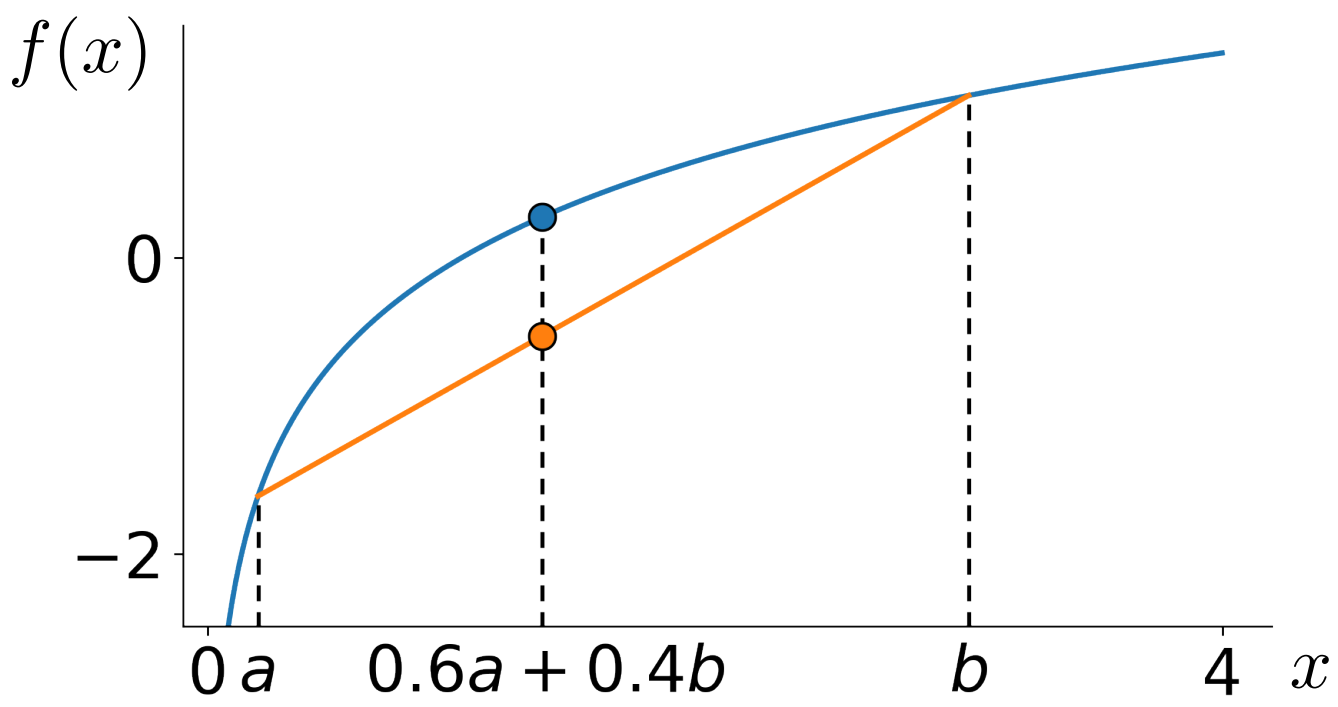
\includegraphics[width=0.6\columnwidth]{exp/concave.png}
    \caption{Concave Function\\\textcolor{BGpurple}{Ref: \cite{bayesML}}}
\end{figure}
$$\text{Jensen's Inequality:~~}f\left(\mathbb{E}_{p(t)}(t)\right)\geq \mathbb{E}_{p(t)}f(t)$$
\end{frame}
%%%%%%%%%%%%%%%%%%%%%%%%%%%%%%%%%%%%%%%%%%%%%%%%%%%%%%%%%%%%%
\begin{frame}{Preliminary: Kullback-Leibler (KL) divergence}

$$\mathcal{KL}(P\parallel Q)=\int_{-\infty}^{\infty}p(x)\log\frac{p(x)}{q(x)}dx$$

\begin{itemize}
  \item A way to compare distributions
  \item Not a proper distance
\end{itemize}

\begin{figure}
    \centering
    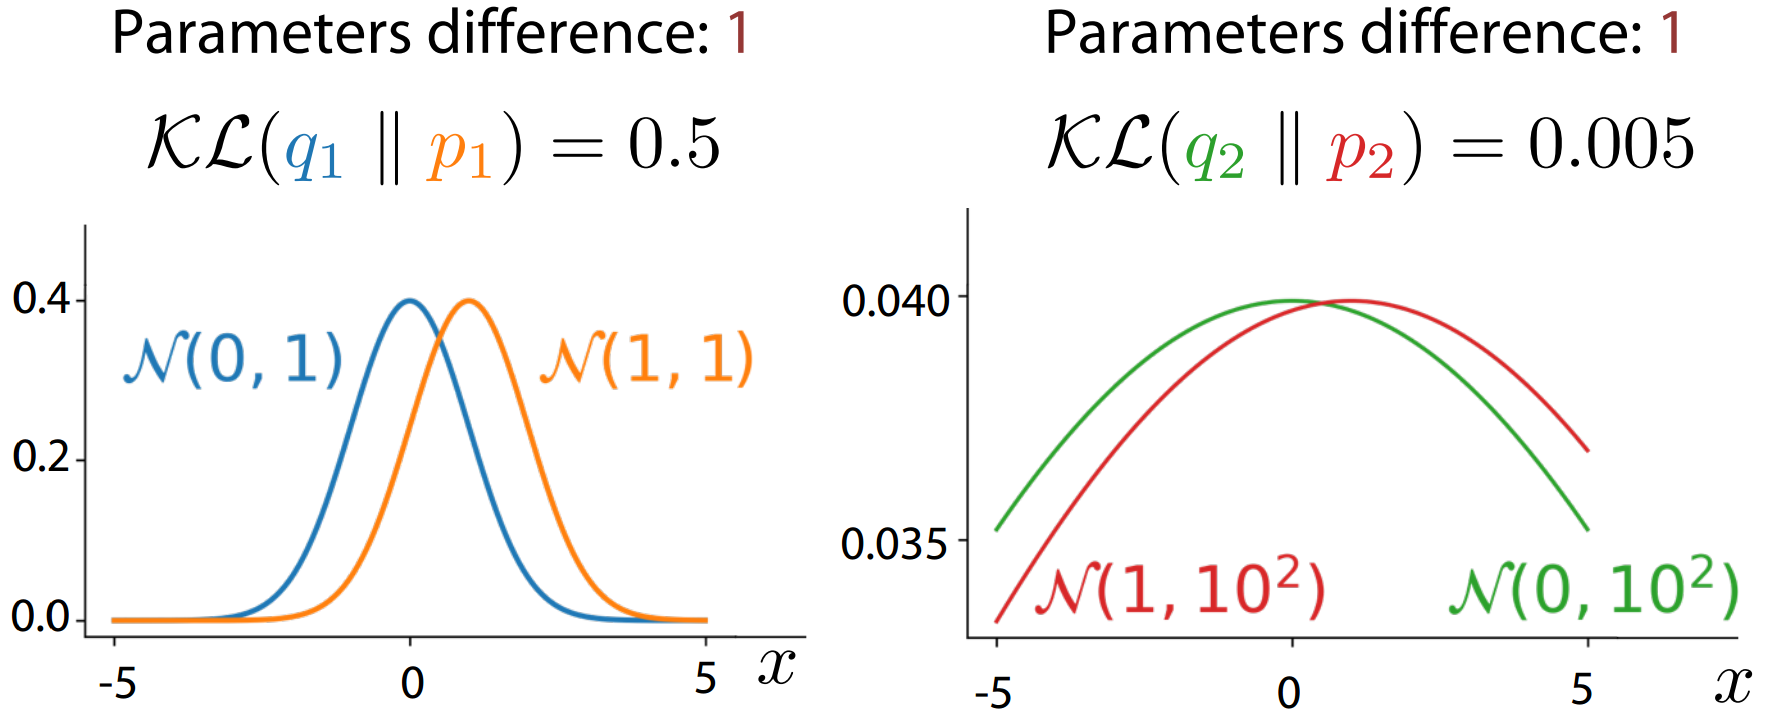
\includegraphics[width=0.9\columnwidth]{exp/KL.png}
    \caption{\textcolor{BGpurple}{Ref: \cite{bayesML}}}
\end{figure}

\end{frame}
%%%%%%%%%%%%%%%%%%%%%%%%%%%%%%%%%%%%%%%%%%%%%%%%%%%%%%%%%%%%%
% \begin{frame}{title}{subtitle}
%   \begin{proof}
%     \begin{enumerate}
%       \item<1-> &1
%       \item<2-> &2
%       \item<3-> &3
%       \item<4-> &4 \qedhere
%     \end{enumerate}
%   \end{proof}
% \end{frame}
%%%%%%%%%%%%%%%%%%%%%%%%%%%%%%%%%%%%%%%%%%%%%%%%%%%%%%%%%%%%%
{%BACKGROUND START
\usebackgroundtemplate{
\includegraphics[width=\paperwidth]{fig/BG.png}}
\begin{frame}
\begin{center}
{\bf\LARGE Variational Lower Bound}\\
~\\
\textit{a.k.a.} Evidence Lower Bound (ELBO)
\end{center}
\end{frame}
}%BACKGROUND E N D
%%%%%%%%%%%%%%%%%%%%%%%%%%%%%%%%%%%%%%%%%%%%%%%%%%%%%%%%%%%%%\
% \begin{frame}
% The marginal likelihood is composed of a sum over the marginal likelihoods of individual datapoints
% $$\log p_{\theta}(X)=\log p_{\theta}(x(1);\cdots; x(N))
% =\sum_{i=1}^N \log p_{\theta}(x_i)$$
% \end{frame}
%%%%%%%%%%%%%%%%%%%%%%%%%%%%%%%%%%%%%%%%%%%%%%%%%%%%%%%%%%%%%
\begin{frame}{Variational Lower Bound}
\begin{align*}
    \log p_{\mathbf{\theta}}(X)
    &\uncover<1->{=\log\int_{Z} p_{\theta}(X,Z)}\\
    &\uncover<2->{
    =\log\int_{Z} \frac{\textcolor{DeepSkyBlue3}{q_{\phi}(Z)}}{\textcolor{DarkOrange}{q_{\phi}(Z)}}\textcolor{DarkOrange}{p_{\theta}(X,Z)}
    =\log\int_{Z} \textcolor{DeepSkyBlue3}{q_{\phi}(Z)}\frac{\textcolor{DarkOrange}{p_{\theta}(X,Z)}}{\textcolor{DarkOrange}{q_{\phi}(Z)}}}\\
    &\uncover<3->{
    =\log\mathbb{E}_{q_{\phi}(Z)}\frac{p_{\theta}(X,Z)}{q_{\phi}(Z)}} \uncover<4>{\textit{~~then by Jensen's Inequality}}\\
    &\uncover<5->{
    \geq\mathbb{E}_{q_{\phi}(Z)}\log\frac{p_{\theta}(X,Z)}{q_{\phi}(Z)}}\\
    &\uncover<6->{
    \overset{\Delta}{=}\mathcal{L}(\theta,q)}
    \uncover<7->{
    \text{\bf\textcolor{MidnightBlue}{~~Variational Lower Bound, {\it a.k.a.} ELBO}}}
\end{align*}
\end{frame}
%%%%%%%%%%%%%%%%%%%%%%%%%%%%%%%%%%%%%%%%%%%%%%%%%%%%%%%%%%%%%
\begin{frame}{Variational Lower Bound}%{\textit{a.k.a.} Evidence Lower Bound (ELBO)}
Then $\mathcal{L}(\theta,q)$ is referred as \textcolor{DeepPink3}{variational lower bound}, \textit{a.k.a.} evidence lower bound (ELBO), and it always holds true that
$$\log p(X\mid\theta)\geq\mathcal{L}(\theta,q), \text{ for any } q.$$

%Note: $\mathcal{L}(\theta,q)=\mathbb{E}_{q_{\phi}(Z)}\log\frac{p_{\theta}(X,Z)}{q_{\phi}(Z)}$
\end{frame}
%%%%%%%%%%%%%%%%%%%%%%%%%%%%%%%%%%%%%%%%%%%%%%%%%%%%%%%%%%%%%
\begin{frame}{Understanding Variational Lower Bound}
\begin{figure}[htbp]
  \centering
  \foreach \x in {1,...,5} {
  \includegraphics<\x>[width=0.64\columnwidth]{gap/gap-\x.png}}
  \caption{\textcolor{BGpurple}{Ref: \cite{bayesML}}}
\end{figure}
\end{frame}
%%%%%%%%%%%%%%%%%%%%%%%%%%%%%%%%%%%%%%%%%%%%%%%%%%%%%%%%%%%%%
\begin{frame}{Understanding Variational Lower Bound}
To calculate the GAP between $\log p_{\theta}(X)$ and $\mathcal{L}(\theta,q)$,%(in order to minimize it),
\begin{align*}
  &\log p_{\theta}(X)-\mathcal{L}(\theta,q)\\
  =&\log p_{\theta}(X)
  -\mathbb{E}_{q_{\phi}(Z)}\log\frac{p_{\theta}(X,Z)}{q_{\phi}(Z)}\\
  =&\mathbb{E}_{q_{\phi}(Z)}\left[
  \log p_{\theta}(X)-\log\frac{p_{\theta}(X,Z)}{q_{\phi}(Z)}\right]\\
  =&\mathbb{E}_{q_{\phi}(Z)}\left
  [\log\frac{p_{\theta}(X)}{p_{\theta}(X,Z)}\cdot q_{\phi}(Z)\right]\\
  =&\mathbb{E}_{q_{\phi}(Z)}\left
  [\log\frac{q_{\phi}(Z)}{p_{\theta}(Z\mid X)}\right]\\
  =&\textcolor{DeepPink3}{\mathcal{KL}(q_{\phi}(Z)\parallel p_{\theta}(Z\mid X))}
\end{align*}
\end{frame}
%%%%%%%%%%%%%%%%%%%%%%%%%%%%%%%%%%%%%%%%%%%%%%%%%%%%%%%%%%%%%
\begin{frame}{Understanding Variational Lower Bound}
$$\textcolor{DeepPink3}{\log p_{\theta}(X)-\mathcal{L}(\theta,q)
=\mathcal{KL}(q_{\phi}(Z)\parallel p_{\theta}(Z\mid X))}$$
\begin{figure}
    \centering
    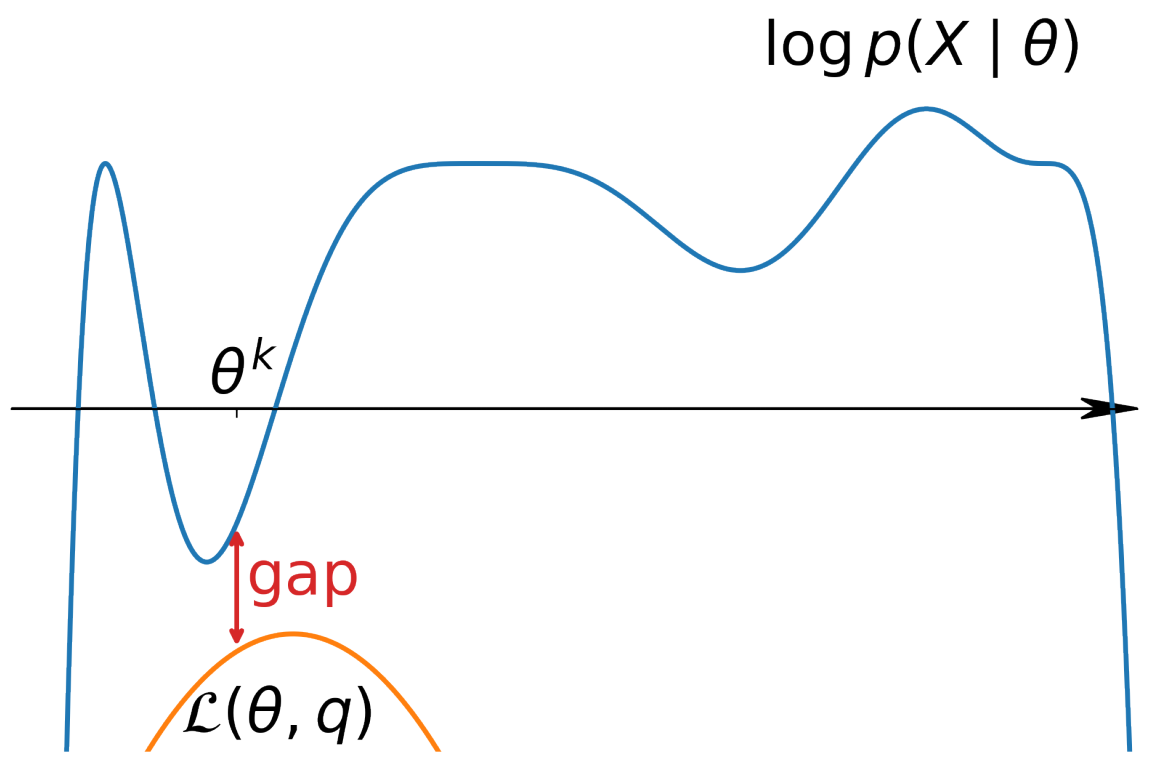
\includegraphics[width=0.64\columnwidth]{gap/gap-GAP.png}
    \caption{\textcolor{BGpurple}{Ref: \cite{bayesML}}}
\end{figure}
\end{frame}
%%%%%%%%%%%%%%%%%%%%%%%%%%%%%%%%%%%%%%%%%%%%%%%%%%%%%%%%%%%%%
{%BACKGROUND START
\usebackgroundtemplate{
\includegraphics[width=\paperwidth]{fig/BG.png}}
\begin{frame}
\begin{center}
{\bf\LARGE Revisiting Variational Lower Bound}\\
~\\
\textit{a.k.a.} Evidence Lower Bound (ELBO)
\end{center}
\end{frame}
}%BACKGROUND E N D
%%%%%%%%%%%%%%%%%%%%%%%%%%%%%%%%%%%%%%%%%%%%%%%%%%%%%%%%%%%%%
\begin{frame}{Revisiting Variational Lower Bound}

\textit{Note: $q_{\phi}(Z\mid X)$ is usually written as $q_{\phi}(Z)$ for simplicity}

\begin{align*}
  \uncover<1->{
   \mathcal{L}(\theta,q)
  =&~\mathbb{E}_{q_{\phi}(Z)}
  \log\frac{p_{\theta}(X,Z)}{q_{\phi}(Z)}}\\
  \uncover<2->{
  =&~\mathbb{E}_{q_{\phi}(Z)}
  \log\frac{p_{\theta}(X\mid Z)p_{\theta}(Z)}{q_{\phi}(Z)}}\\
  \uncover<3->{
  =&~\mathbb{E}_{q_{\phi}(Z)}\log\frac{p_{\theta}(Z)}{q_{\phi}(Z)}
  +\mathbb{E}_{q_{\phi}(Z\mid X)}\log{p_{\theta}(X\mid Z)}}\\
  \uncover<4->{
  =&~
  \textcolor{DeepSkyBlue3}{-
  \mathcal{KL}(q_{\phi}(Z\mid X)\parallel p_{\theta}(Z\mid X))}
  +
  \textcolor{DeepPink3}{
  \mathbb{E}_{q_{\phi}(Z\mid X)}\log{p_{\theta}(X \mid Z)}}}\\
  \uncover<5->{
  =&~
  \text{\textcolor{DeepSkyBlue3}{Regularization}}
  +
  \text{\textcolor{DeepPink3}{Reconstruction}}}
\end{align*}
\end{frame}
%%%%%%%%%%%%%%%%%%%%%%%%%%%%%%%%%%%%%%%%%%%%%%%%%%%%%%%%%%%%%
\begin{frame}{Revisiting Variational Lower Bound}
%
Now we have rewritten $\mathcal{L}(\theta,q)$ into two parts as follows:
%
\begin{align*}
  \mathcal{L}(\theta,q)
  =&~
  \textcolor{DeepSkyBlue3}{-
  \mathcal{KL}(q_{\phi}(Z\mid X)\parallel p_{\theta}(Z\mid X))}
  +
  \textcolor{DeepPink3}{
  \mathbb{E}_{q_{\phi}(Z\mid X)}\log{p_{\theta}(X \mid Z)}}\\
  =&~
  \text{\textcolor{DeepSkyBlue3}{Regularization}}+
  \text{\textcolor{DeepPink3}{Reconstruction}}
\end{align*}
%
Given the evidence $X$ of $N$ samples $x^{(1)},\dots,x^{(N)}$, $\mathcal{L}(\theta,q)$ is calculated by taking the average.
%
\begin{align*}
  \mathcal{L}(\theta,q)
  =&~\sum_{i=1}^{N}
  \textcolor{DeepSkyBlue3}{-
  \mathcal{KL}(q_{\phi}(z| x^{(i)})\parallel p_{\theta}(z| x^{(i)}))}
  +
  \textcolor{DeepPink3}{
  \mathbb{E}_{q_{\phi}(z|x^i)}\log{p_{\theta}(x^{(i)}
  | z)}}
\end{align*}

\end{frame}
%%%%%%%%%%%%%%%%%%%%%%%%%%%%%%%%%%%%%%%%%%%%%%%%%%%%%%%%%%%%%
\begin{frame}{Revisiting Variational Lower Bound}
%
\begin{align*}
  \mathcal{L}(\theta,q)
  =&~\sum_{i=1}^{N}
  \textcolor{DeepSkyBlue3}{-
  \mathcal{KL}(q_{\phi}(z| x^{(i)})\parallel p_{\theta}(z| x^{(i)}))}
  +
  \textcolor{DeepPink3}{
  \mathbb{E}_{q_{\phi}(z|x^i)}\log{p_{\theta}(x^{(i)}
  | z)}}
\end{align*}
%
\indent Take $x^{(i)}, i\in{1,\dots,N}$ for example:
%
\begin{figure}
    \centering
    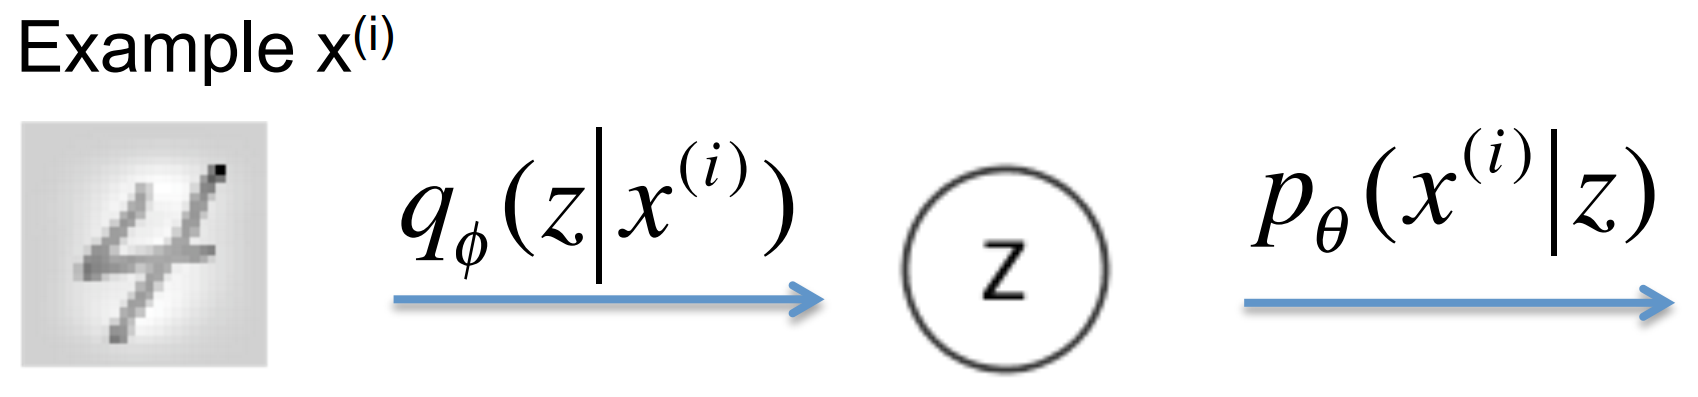
\includegraphics[width=0.6\columnwidth]{exp/regu+reco.png}
\end{figure}
\begin{center}
{\small \textcolor{BGpurple}
{Ref: \url{https://tensorchiefs.github.io/bbs/files/vae.pdf}}}
\end{center}
\noindent\textcolor{DeepSkyBlue3}{\bf Regularization}:
  $p(z)$ is usually a simple prior $\mathcal{N}(0,1)$
\noindent\textcolor{DeepPink3}{\bf Reconstruction} quality: $\log(1)$ if $x^{(i)}$ gets always reconstructed perfectly ($z$ produces $x^{(i)}$)
% \begin{itemize}
%   \item[] \textcolor{DeepSkyBlue3}{\bf Regularization}:
%   $p(z)$ is usually a simple prior $\mathcal{N}(0,1)$
%   \item[] \textcolor{DeepPink3}{\bf Reconstruction} quality: $\log(1)$ if $x^{(i)}$ gets always reconstructed perfectly ($z$ produces $x^{(i)}$)
% \end{itemize}
\end{frame}
%%%%%%%%%%%%%%%%%%%%%%%%%%%%%%%%%%%%%%%%%%%%%%%%%%%%%%%%%%%%%
\begin{frame}{Calculation of the Regularization}
Common assumptions
\begin{itemize}
  \item use $\mathcal{N}(0,1)$ as prior for $p(Z)$
  \item $q(Z\mid X)$ is Gaussian with parameters $(\mu(X),\sigma(X))$ determined by Neural Networks
\end{itemize}
~\\
The \textcolor{DeepSkyBlue3}{ Regularization} term can be calculated analytically:
\begin{align*}
&-\mathcal{KL}(q_{\phi}(Z\mid X)\parallel p_{\theta}(Z\mid X))\\
&=\frac{1}{2} \sum_{i=1}^N \sum_{s=1}^D
\left(1+\log(\sigma(z_s^{{(i)}^2}))
-\mu_s^{{(i)}^2}
-\sigma_s^{{(i)}^2})\right)
\end{align*}

$N$ is the number of samples;
$D$ is the number of latent variables.
\begin{align*}
\end{align*}
\end{frame}
%%%%%%%%%%%%%%%%%%%%%%%%%%%%%%%%%%%%%%%%%%%%%%%%%%%%%%%%%%%%%
\begin{frame}{Sampling to calculate the Reconstruction}
Approximating $\mathbb{E}_{q_{\phi}}$ with sampling from the distribution $q(Z\mid X)$

$$\mathbb{E}_{q_{\phi}(Z\mid X)}\log{p_{\theta}(X \mid Z)}
= \frac{1}{N\cdot J} \sum_{i=1}^N \sum_{j=1}^J \log p_{\theta}(x^{(i)} \mid z^{(i,j)})$$

\begin{itemize}
    \item $\textcolor{DeepPink3}{\bf -}\log{p_{\theta}(x_{(i)} \mid z^{(i,j)})}$ can use L2 loss \& cross entropy loss, \textit{etc.}
    \item $J$ is the number of $z$ sampled from $q(z\mid x^{(i)})$
\end{itemize}

\begin{figure}
    \centering
    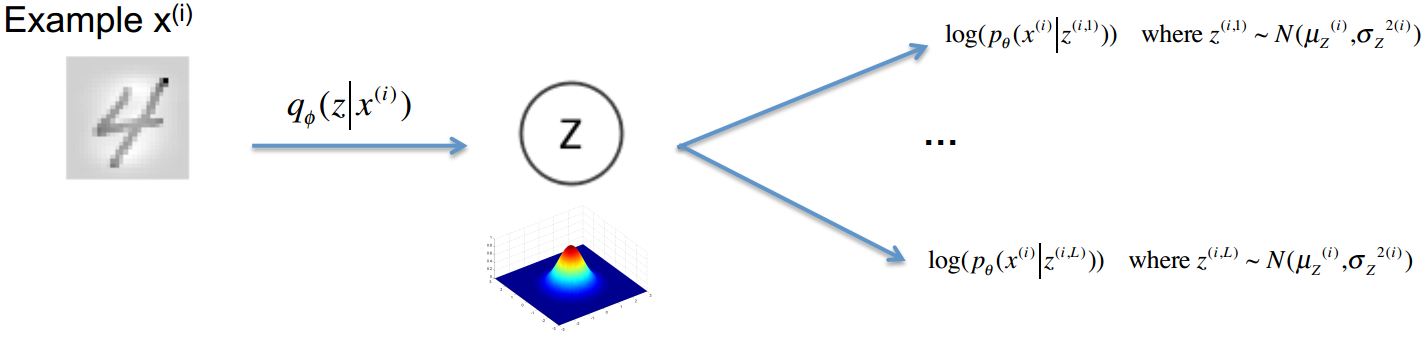
\includegraphics[width=0.95\columnwidth]{exp/regu+reco-2.png}
    \caption{\small \textcolor{BGpurple}
{Ref: \url{https://tensorchiefs.github.io/bbs/files/vae.pdf}}}
\end{figure}

\end{frame}
%%%%%%%%%%%%%%%%%%%%%%%%%%%%%%%%%%%%%%%%%%%%%%%%%%%%%%%%%%%%%
\begin{frame}{Revisiting ELBO: Putting it altogether}

We have now arrived at
\begin{align*}
 \mathcal{L}(\theta,q)
&=\frac{1}{2} \sum_{i=1}^N \sum_{s=1}^D
 \left(1+\log(\sigma(z_s^{{(i)}^2}))
 -\mu_s^{{(i)}^2}
 -\sigma_s^{{(i)}^2})\right)\\
&+\frac{1}{N\cdot J} \sum_{i=1}^N \sum_{j=1}^J
 \log p_{\theta}(x^{(i)} \mid z^{(i,j)})
\end{align*}

Recall that
$$\textcolor{DeepPink3}{\log p_{\theta}(X)-\mathcal{L}(\theta,q)
=\mathcal{KL}(q_{\phi}(Z)\parallel p_{\theta}(X\mid Z))}$$

Use mini batch gradient decent to perform optimization.
$$\text{maximize } \mathcal{L}(\theta,q) \text{ (ELBO)} \Longleftrightarrow \text{minimize~~} \mathcal{KL}(q_{\phi}(Z)\parallel p_{\theta}(X\mid Z))$$

\end{frame}
%%%%%%%%%%%%%%%%%%%%%%%%%%%%%%%%%%%%%%%%%%%%%%%%%%%%%%%%%%%%%
{%BACKGROUND START
\usebackgroundtemplate{
\includegraphics[width=\paperwidth]{fig/BG.png}}
\begin{frame}
\begin{center}
{\bf\LARGE Reparameterization Trick}
\end{center}
\end{frame}
}%BACKGROUND E N D
%%%%%%%%%%%%%%%%%%%%%%%%%%%%%%%%%%%%%%%%%%%%%%%%%%%%%%%%%%%%%
\begin{frame}{Reparameterization Trick}
\begin{figure}
    \centering
    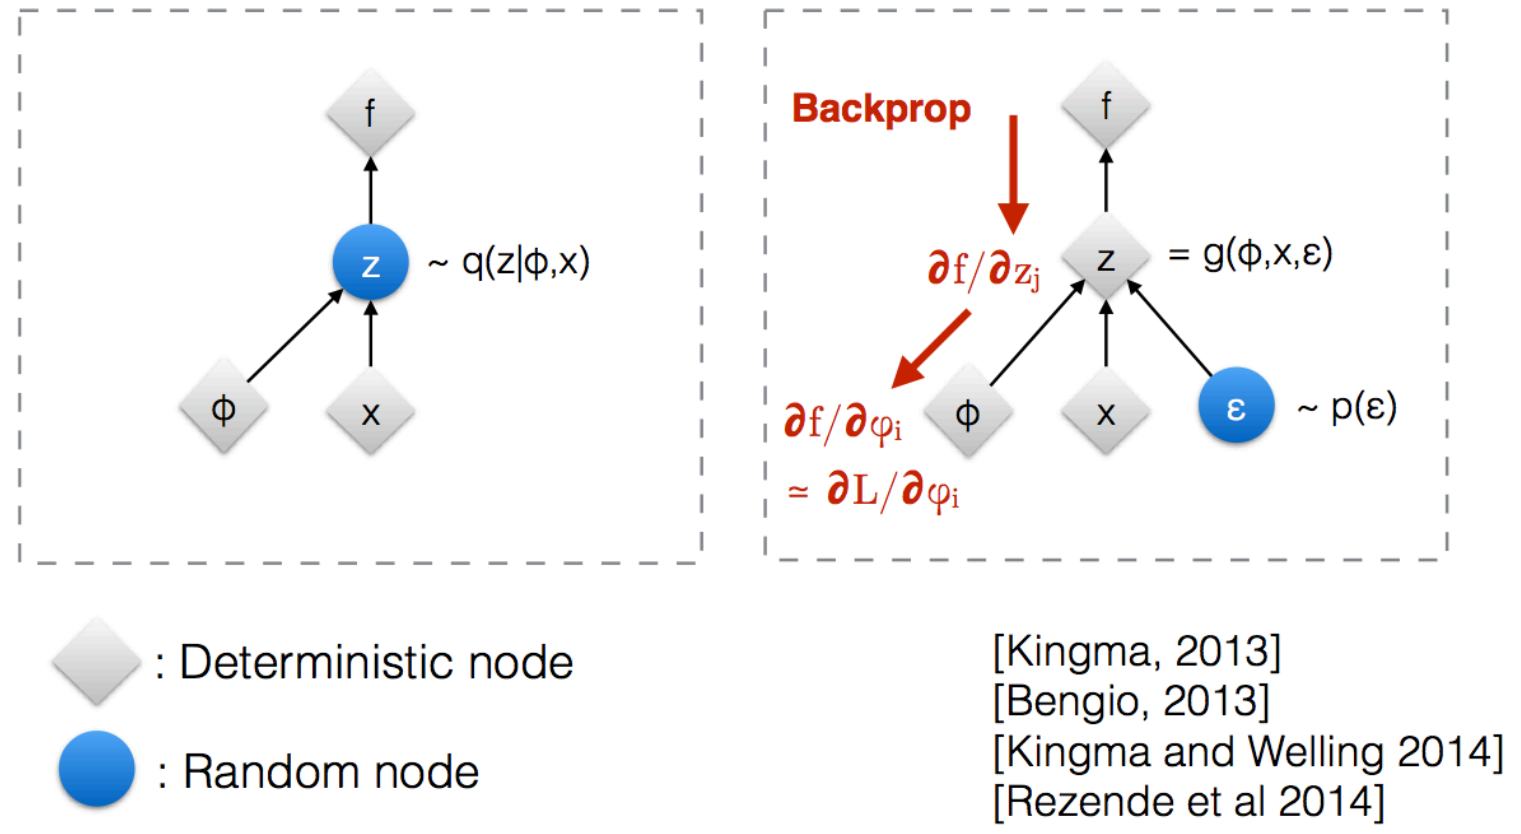
\includegraphics[width=0.9\columnwidth]{exp/reparam-pic.png}
\end{figure}
\end{frame}
%%%%%%%%%%%%%%%%%%%%%%%%%%%%%%%%%%%%%%%%%%%%%%%%%%%%%%%%%%%%%
\begin{frame}{Reparameterization Trick}
\begin{figure}
    \centering
    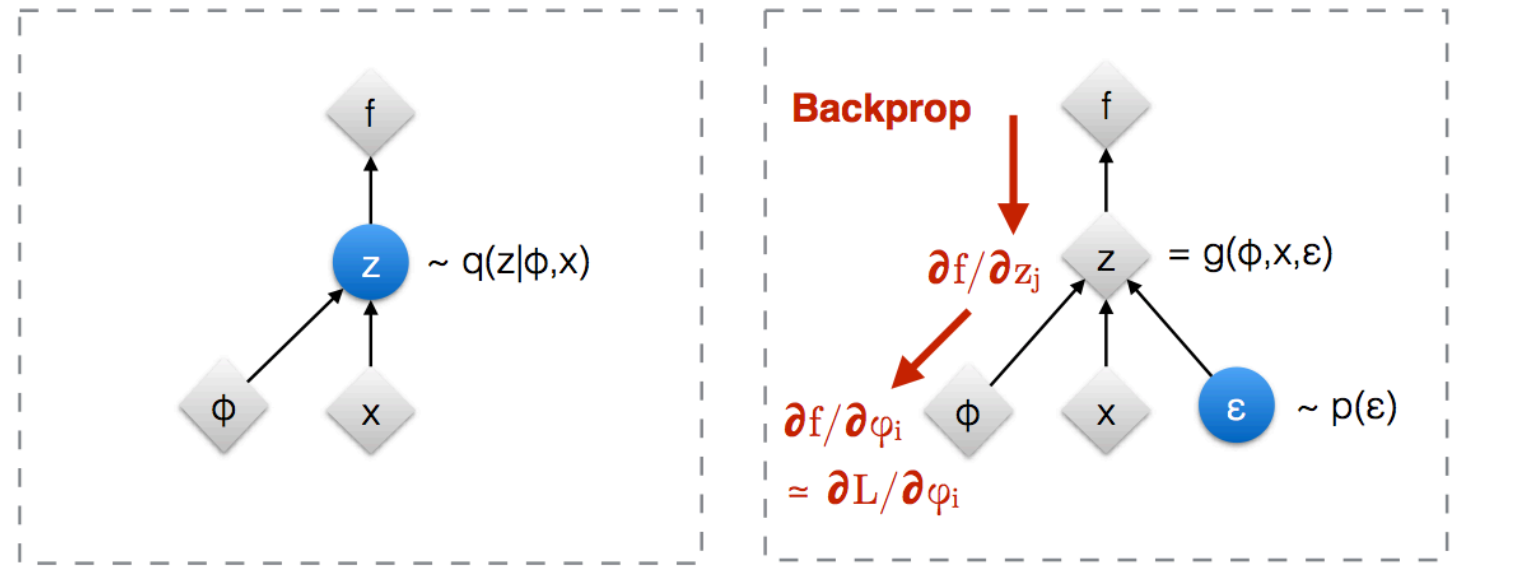
\includegraphics[width=0.9\columnwidth]{exp/reparam-pic-2.png}
\end{figure}
% \begin{align*}
% \mathcal{L}(\theta, \phi)
% &\approx \frac{1}{2} \sum_{d=1}^{D} \left(1 + \log(\sigma_{\phi,d}^2(x)) - \mu_{\phi, d}^2(x) - \sigma_{\phi, d}^2(x) \right) \\
% &+ \frac{1}{L} \sum_{l=1}^{L} \log p_{\theta}(x|z^{(l)}) \label{eqnVAVB} \\
% \text{where} &\,\,\, z^{(l)} = \mu_{\phi}(x) + \epsilon \odot \sigma_{\phi}(x) \,\,\,\text{and}\,\,\, \epsilon^{(l)} \sim \mathcal{N}(\epsilon; 0, \mathbf{I}) \notag
% \end{align*}
\begin{align*}
 \mathcal{L}(\theta,q)
&=\frac{1}{2} \sum_{i=1}^N \sum_{s=1}^D
 \left(1+\log(\sigma(z_{\phi,s}^{{(i)}^2}))
 -\mu_{\phi,s}^{{(i)}^2}
 -\sigma_{\phi,s}^{{(i)}^2})\right)\\
&+\frac{1}{N\cdot J} \sum_{i=1}^N \sum_{j=1}^J
 \log p_{\theta}(x^{(i)} \mid z^{(i,j)})\\
 \text{where}
&\,\,\, z^{(l)} = \mu_{\phi}(x) + \epsilon \odot \sigma_{\phi}(x) \,\,\,\text{and}\,\,\, \epsilon^{(l)} \sim \mathcal{N}(\epsilon; 0, \mathbf{I})
\end{align*}
\end{frame}
%%%%%%%%%%%%%%%%%%%%%%%%%%%%%%%%%%%%%%%%%%%%%%%%%%%%%%%%%%%%%
{%BACKGROUND START
\usebackgroundtemplate{
\includegraphics[width=\paperwidth]{fig/BG.png}}
\begin{frame}
\begin{center}
{\bf\LARGE VAE Structure}
\end{center}
\end{frame}
}%BACKGROUND E N D
%%%%%%%%%%%%%%%%%%%%%%%%%%%%%%%%%%%%%%%%%%%%%%%%%%%%%%%%%%%%%
\begin{frame}{VAE Structure}
\begin{figure}
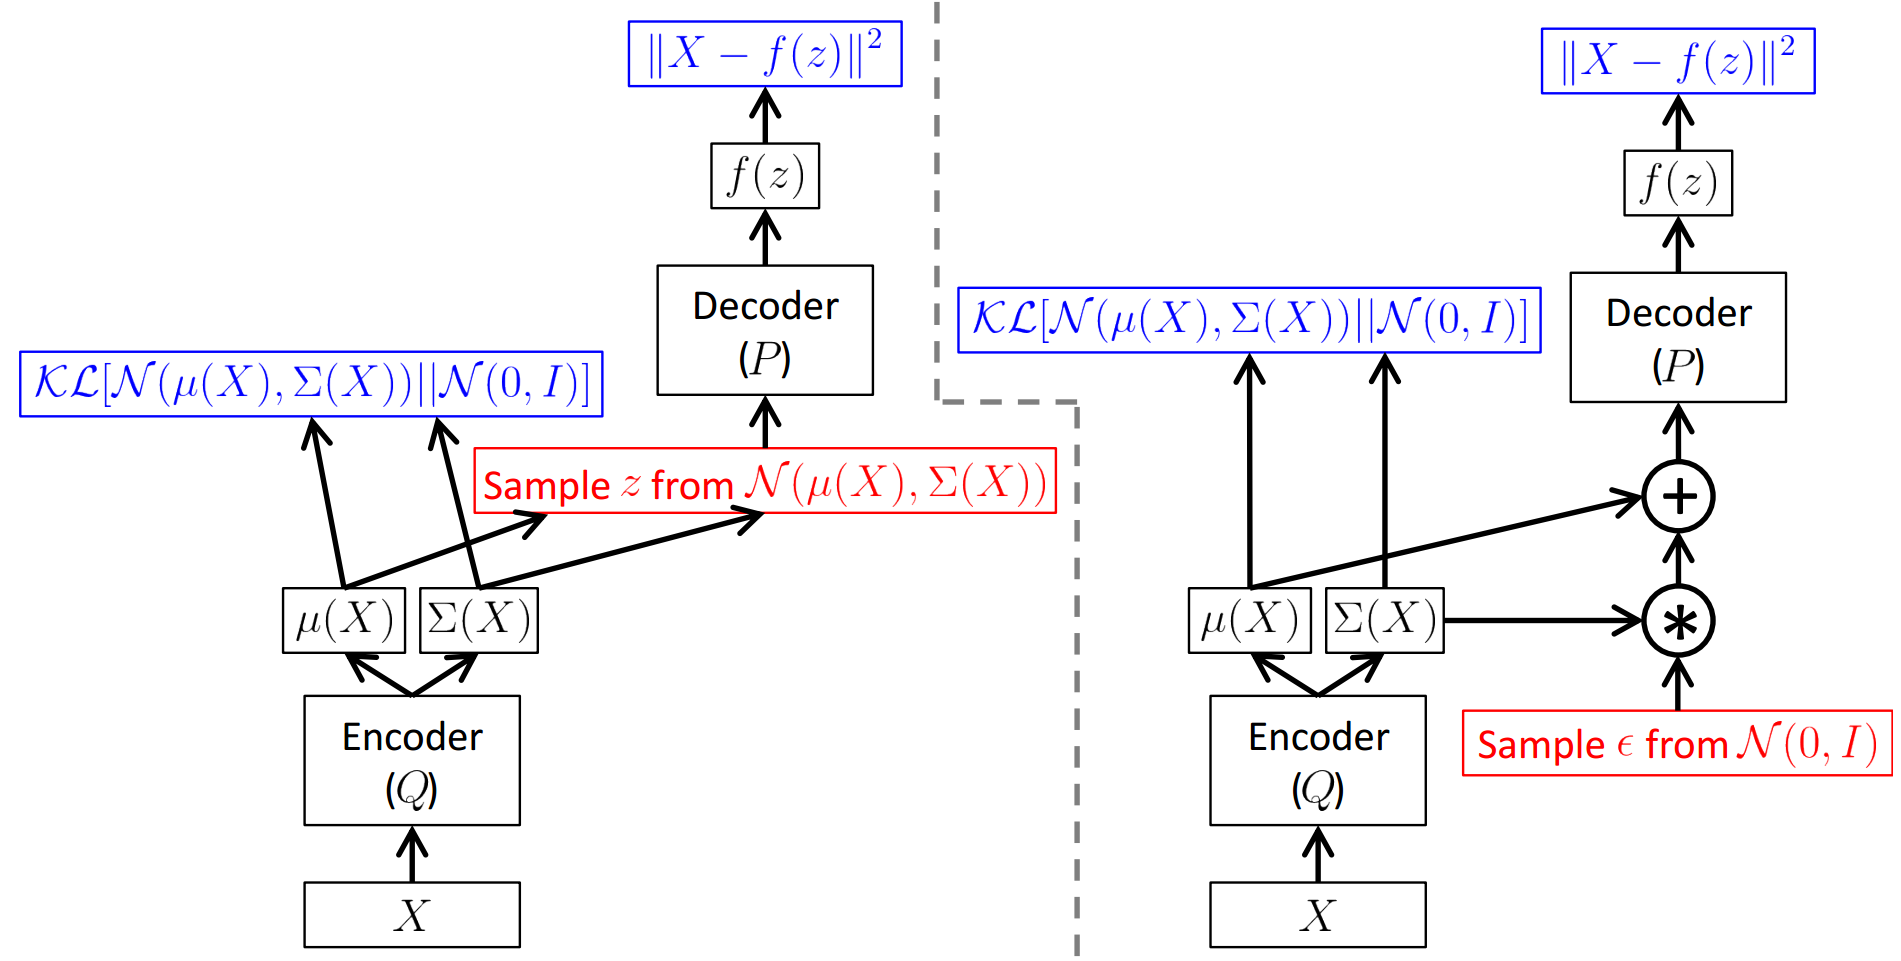
\includegraphics[width=0.95\columnwidth]{fig/vae_paper.png}
\begin{spacing}{1.5}
\textcolor{BGpurple}{\small
Ref: \citet[Tutorial on Variational Autoencoders]{doersch2016tutorial}}
\end{spacing}
\end{figure}
\end{frame}
%%%%%%%%%%%%%%%%%%%%%%%%%%%%%%%%%%%%%%%%%%%%%%%%%%%%%%%%%%%%%
\begin{frame}{VAE Structure}{\textit{e.g.} use a multi-layer perception (MLP) as en/decoder}
\begin{figure}
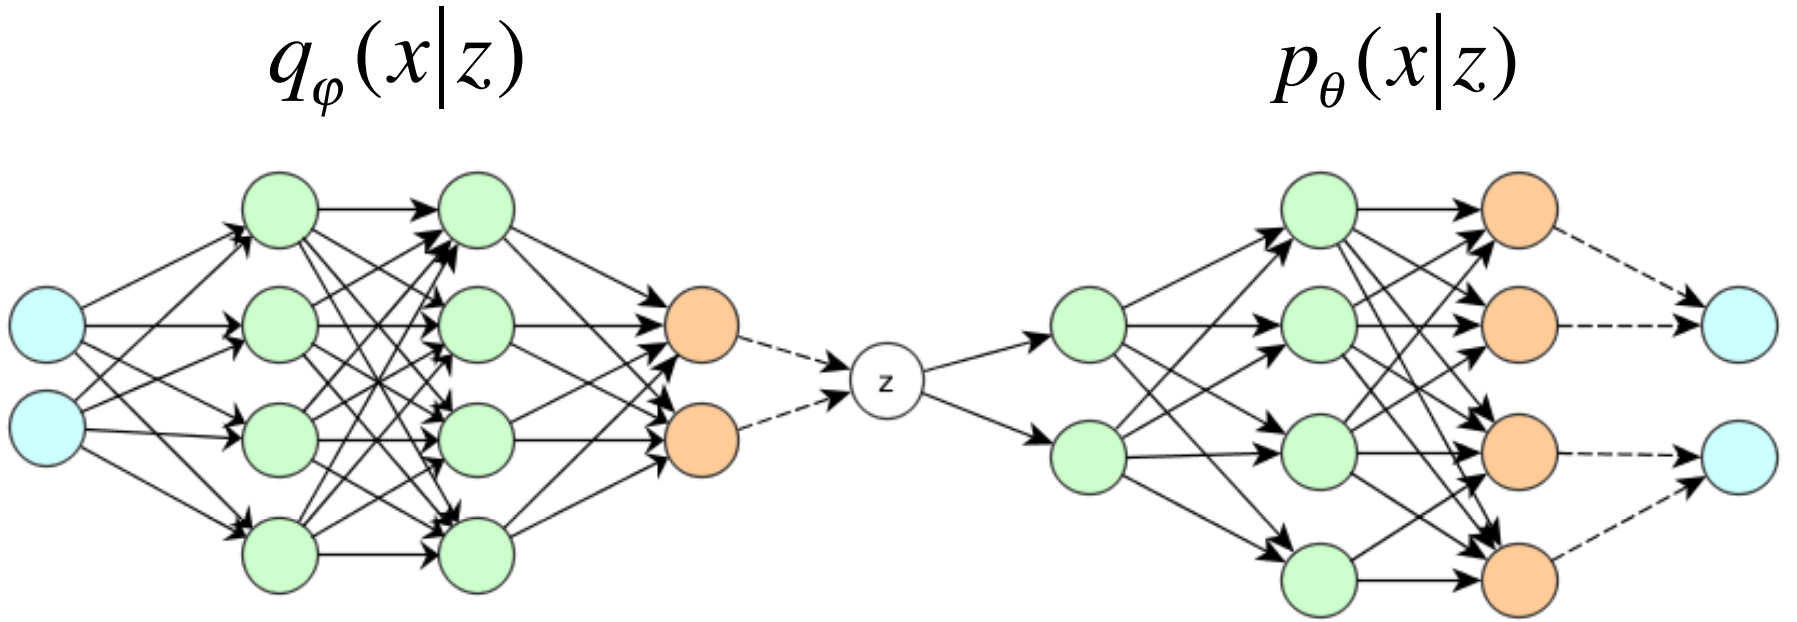
\includegraphics[width=0.9\columnwidth]{exp/vae-str.png}%{fig/vaemlp_vae.png}
\begin{spacing}{1.5}
{\textcolor{BGpurple}
{\small Ref: \url{https://tensorchiefs.github.io/bbs/files/vae.pdf}}}
% \textcolor[RGB]{185 181 205}{Ref: \url{https://zhuanlan.zhihu.com/p/25401928}}
\end{spacing}
\end{figure}
\end{frame}
%%%%%%%%%%%%%%%%%%%%%%%%%%%%%%%%%%%%%%%%%%%%%%%%%%%%%%%%%%%%%
{%BACKGROUND START
\usebackgroundtemplate{
\includegraphics[width=\paperwidth]{fig/BG.png}}
\begin{frame}
\begin{center}
{\bf\LARGE VAE Experiments on MINST}
\end{center}
\end{frame}
}%BACKGROUND E N D
%%%%%%%%%%%%%%%%%%%%%%%%%%%%%%%%%%%%%%%%%%%%%%%%%%%%%%%%%%%%%
\begin{frame}{2D Digits Manifold}
\begin{minipage}[c]{.03\textwidth}~\\\end{minipage}
\begin{minipage}[c]{.47\textwidth}
 \begin{figure}
  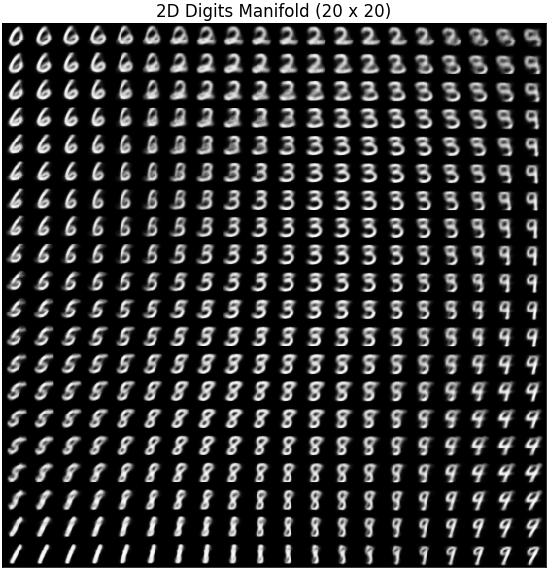
\includegraphics[width=\columnwidth]{fig/x_xent_latent_2_ep_20_n_57.png}
  \caption{VAE (MLP with 2D latent space)}
  \begin{center}
  \textcolor[RGB]{185 181 205}{\tiny code: \url{https://github.com/ThitherShore/VAE-toy/blob/master/vae.py}}
  \end{center}
 \end{figure}
\end{minipage}
\begin{minipage}[c]{.05\textwidth}~\\\end{minipage}
\begin{minipage}[c]{.4\textwidth}
Linearly spaced coordinates on the unit square were transformed through the inverse CDF of the Gaussian to produce values of the latent variables $z$, since the prior of the latent space is Gaussian.
\end{minipage}
\end{frame}
%%%%%%%%%%%%%%%%%%%%%%%%%%%%%%%%%%%%%%%%%%%%%%%%%%%%%%%%%%%%%
\begin{frame}{Image Reconstrution and Denoising}
\begin{figure}[htbp]
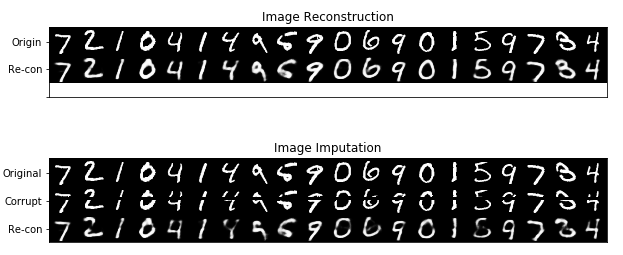
\includegraphics[width=0.95\columnwidth]{fig/i_re_latent_20_ep_70.png}
\caption{Latent = 20, Epochs = 70}
\end{figure}
\begin{center}
\textcolor[RGB]{185 181 205}{\small code: \url{https://github.com/ThitherShore/VAE-toy/blob/master/vae.py}}
\end{center}
\end{frame}
%%%%%%%%%%%%%%%%%%%%%%%%%%%%%%%%%%%%%%%%%%%%%%%%%%%%%%%%%%%%%
% \begin{frame}{2D Latent Space}
% \begin{figure}[htbp]
%   \centering
%   \foreach \x/\y in {1/3,2/5,3/10,4/33,5/53,6/59} {
%   \includegraphics<\x>[width=0.7\columnwidth]{fig/z_xent_latent_2_ep_\y.png}}
%   \caption{2D Latent Space: epoch \y}
% \end{figure}
% \end{frame}
%%%%%%%%%%%%%%%%%%%%%%%%%%%%%%%%%%%%%%%%%%%%%%%%%%%%%%%%%%%%%
\begin{frame}{2D Latent Space}
\begin{figure}[htbp] \centering
\subfigure[epoch = 3]{ \label{fig:a}
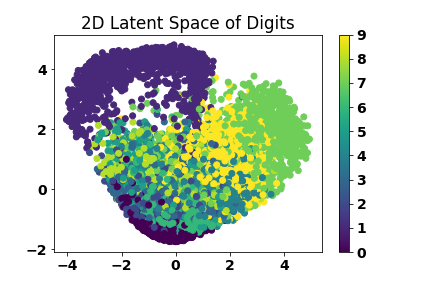
\includegraphics[width=0.3\columnwidth]{fig/z_xent_latent_2_ep_3.png}
}
\subfigure[epoch = 5]{ \label{fig:b}
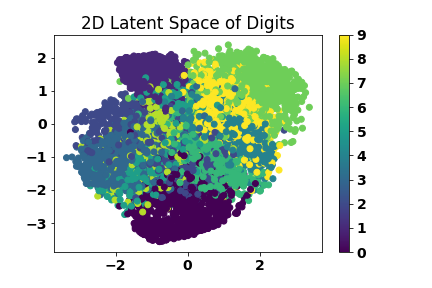
\includegraphics[width=0.3\columnwidth]{fig/z_xent_latent_2_ep_5.png}
}
\subfigure[epoch = 10]{ \label{fig:a}
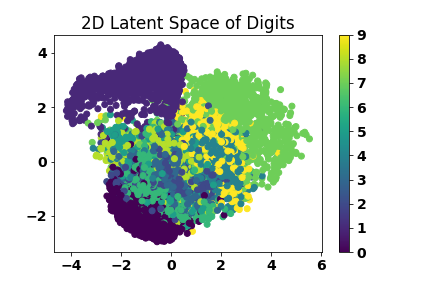
\includegraphics[width=0.3\columnwidth]{fig/z_xent_latent_2_ep_10.png}
}
\subfigure[epoch = 30]{ \label{fig:b}
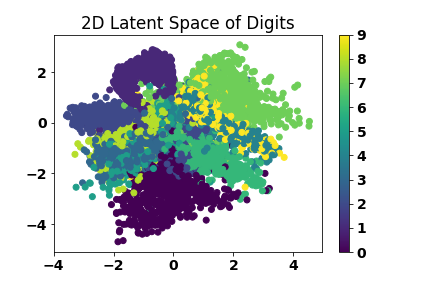
\includegraphics[width=0.3\columnwidth]{fig/z_xent_latent_2_ep_33.png}
}
\subfigure[epoch = 50]{ \label{fig:a}
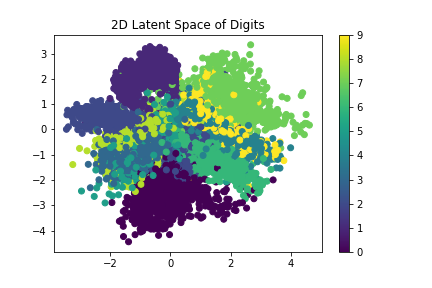
\includegraphics[width=0.3\columnwidth]{fig/z_xent_latent_2_ep_53.png}
}
\subfigure[epoch = 60]{ \label{fig:b}
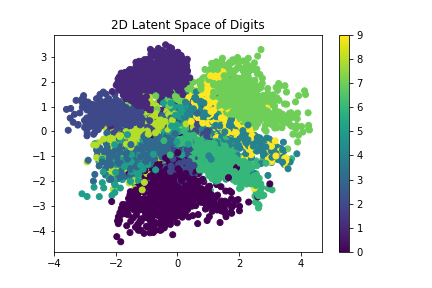
\includegraphics[width=0.32\columnwidth]{fig/z_xent_latent_2_ep_59.png}
}
\caption{2D Latent Space over Epochs}
\textcolor[RGB]{185 181 205}{\small code: \url{https://github.com/ThitherShore/VAE-toy/blob/master/vae.py}}
\end{figure}
\end{frame}
%%%%%%%%%%%%%%%%%%%%%%%%%%%%%%%%%%%%%%%%%%%%%%%%%%%%%%%%%%%%%
\begin{frame}{3D Latent Space}
\begin{figure}[htbp]
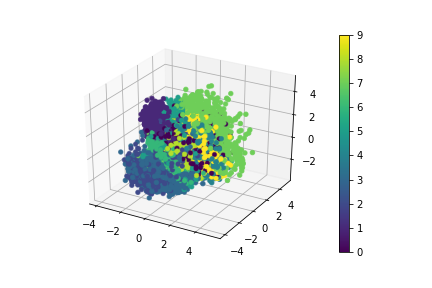
\includegraphics[width=0.9\columnwidth]{fig/3d.png}
\caption{Latent = 3, Epochs = 70}
\textcolor[RGB]{185 181 205}{\small code: \url{https://github.com/ThitherShore/VAE-toy/blob/master/vae.py}}
\end{figure}
\end{frame}
%%%%%%%%%%%%%%%%%%%%%%%%%%%%%%%%%%%%%%%%%%%%%%%%%%%%%%%%%%%%%
\begin{frame}{Loss over Epochs}
\begin{figure}[htbp] \centering
\subfigure[Loss = KL loss + cross entropy]{ \label{fig:a}
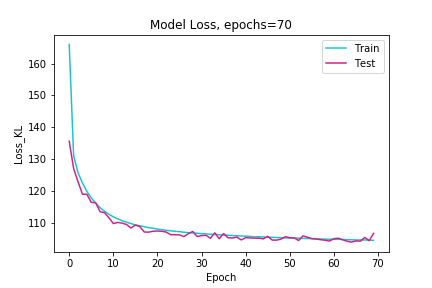
\includegraphics[width=0.47\columnwidth]{fig/loss_xent_latent_20_ep_70.png}
}
\subfigure[KL Loss]{ \label{fig:b}
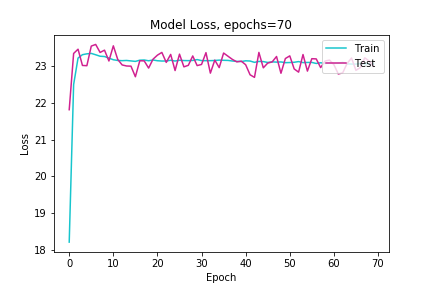
\includegraphics[width=0.47\columnwidth]{fig/loss_kl_xent_latent_20_ep_70.png}
}
\caption{Latent = 20, Epochs = 70}
\textcolor[RGB]{185 181 205}{\small code: \url{https://github.com/ThitherShore/VAE-toy/blob/master/vae.py}}
\end{figure}
\end{frame}
%%%%%%%%%%%%%%%%%%%%%%%%%%%%%%%%%%%%%%%%%%%%%%%%%%%%%%%%%%%%%
\begin{frame}{Compare Multiple Experiments}
\begin{figure}
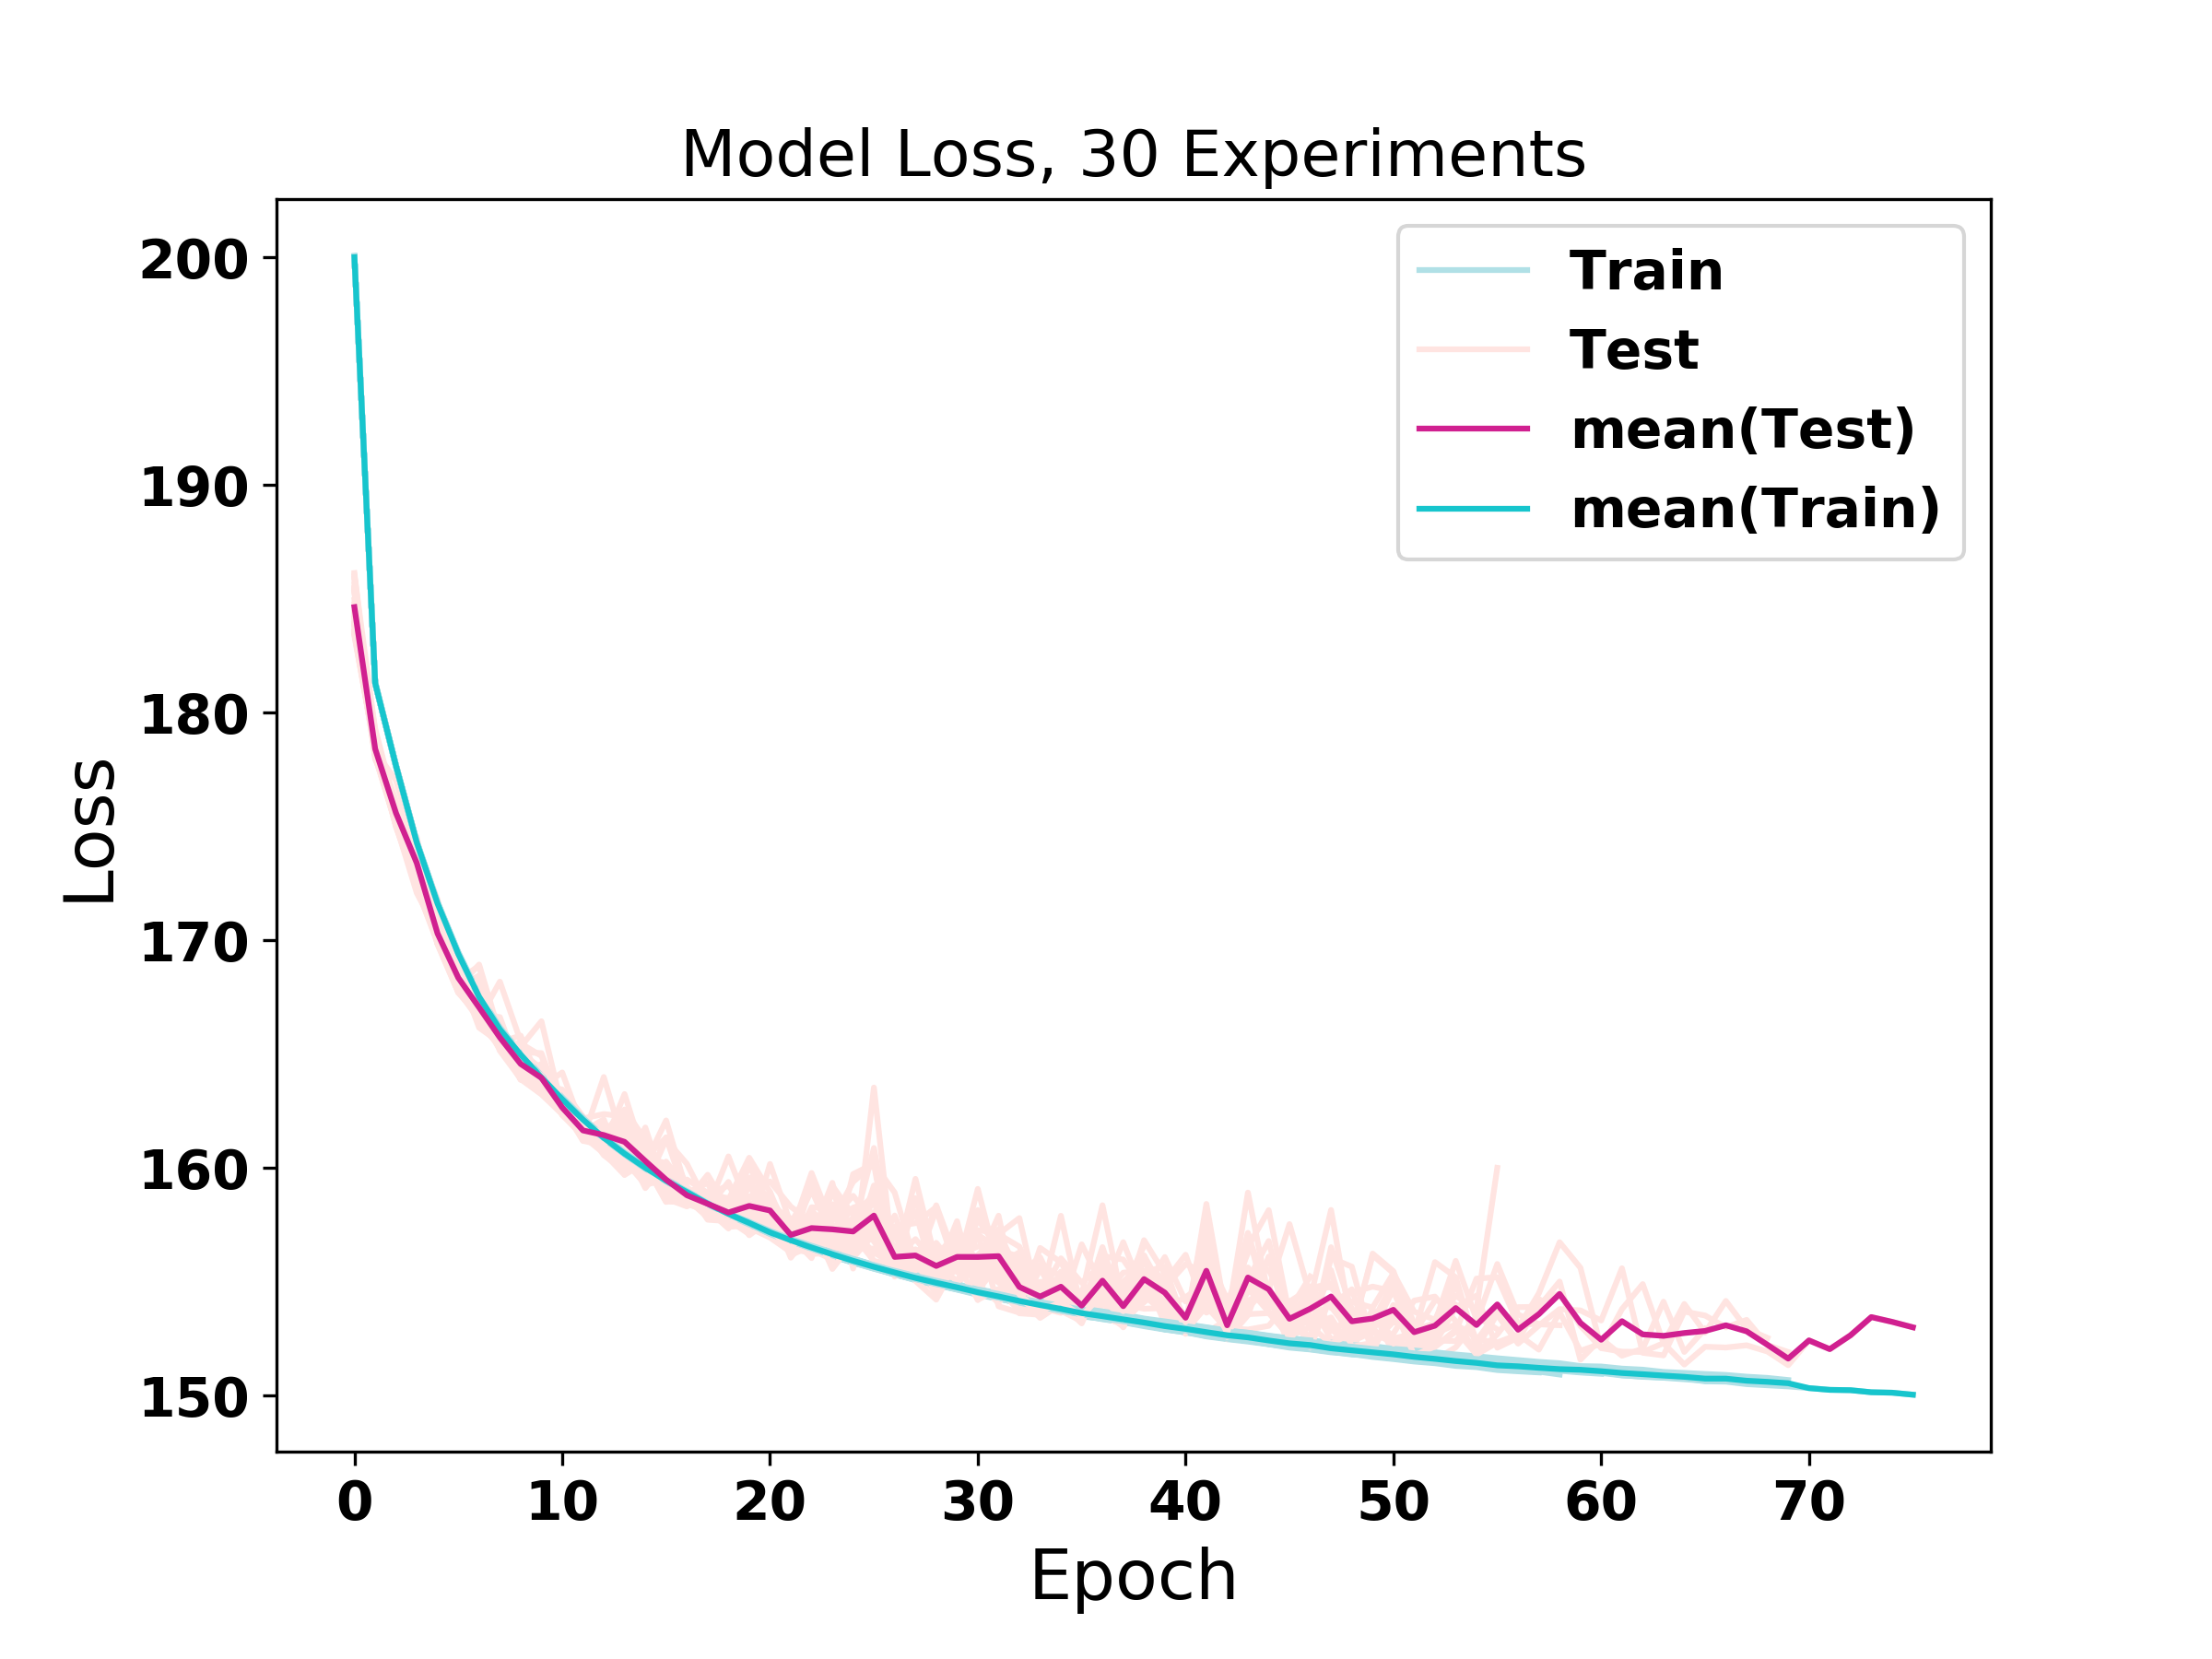
\includegraphics[width=0.7\columnwidth]{fig/loss_30_exps.png}
\caption{Latent = 2, 30 Experiments}
\textcolor[RGB]{185 181 205}{\scriptsize code: \url{https://github.com/ThitherShore/VAE-toy/blob/master/exps\_multiple.py}}
\end{figure}
\end{frame}
%%%%%%%%%%%%%%%%%%%%%%%%%%%%%%%%%%%%%%%%%%%%%%%%%%%%%%%%%%%%%
\begin{frame}{Different Latent Dimensions}
\begin{figure}[htbp] \centering
\subfigure[{EarlyStooping: patience = 5}]{ \label{fig:a}
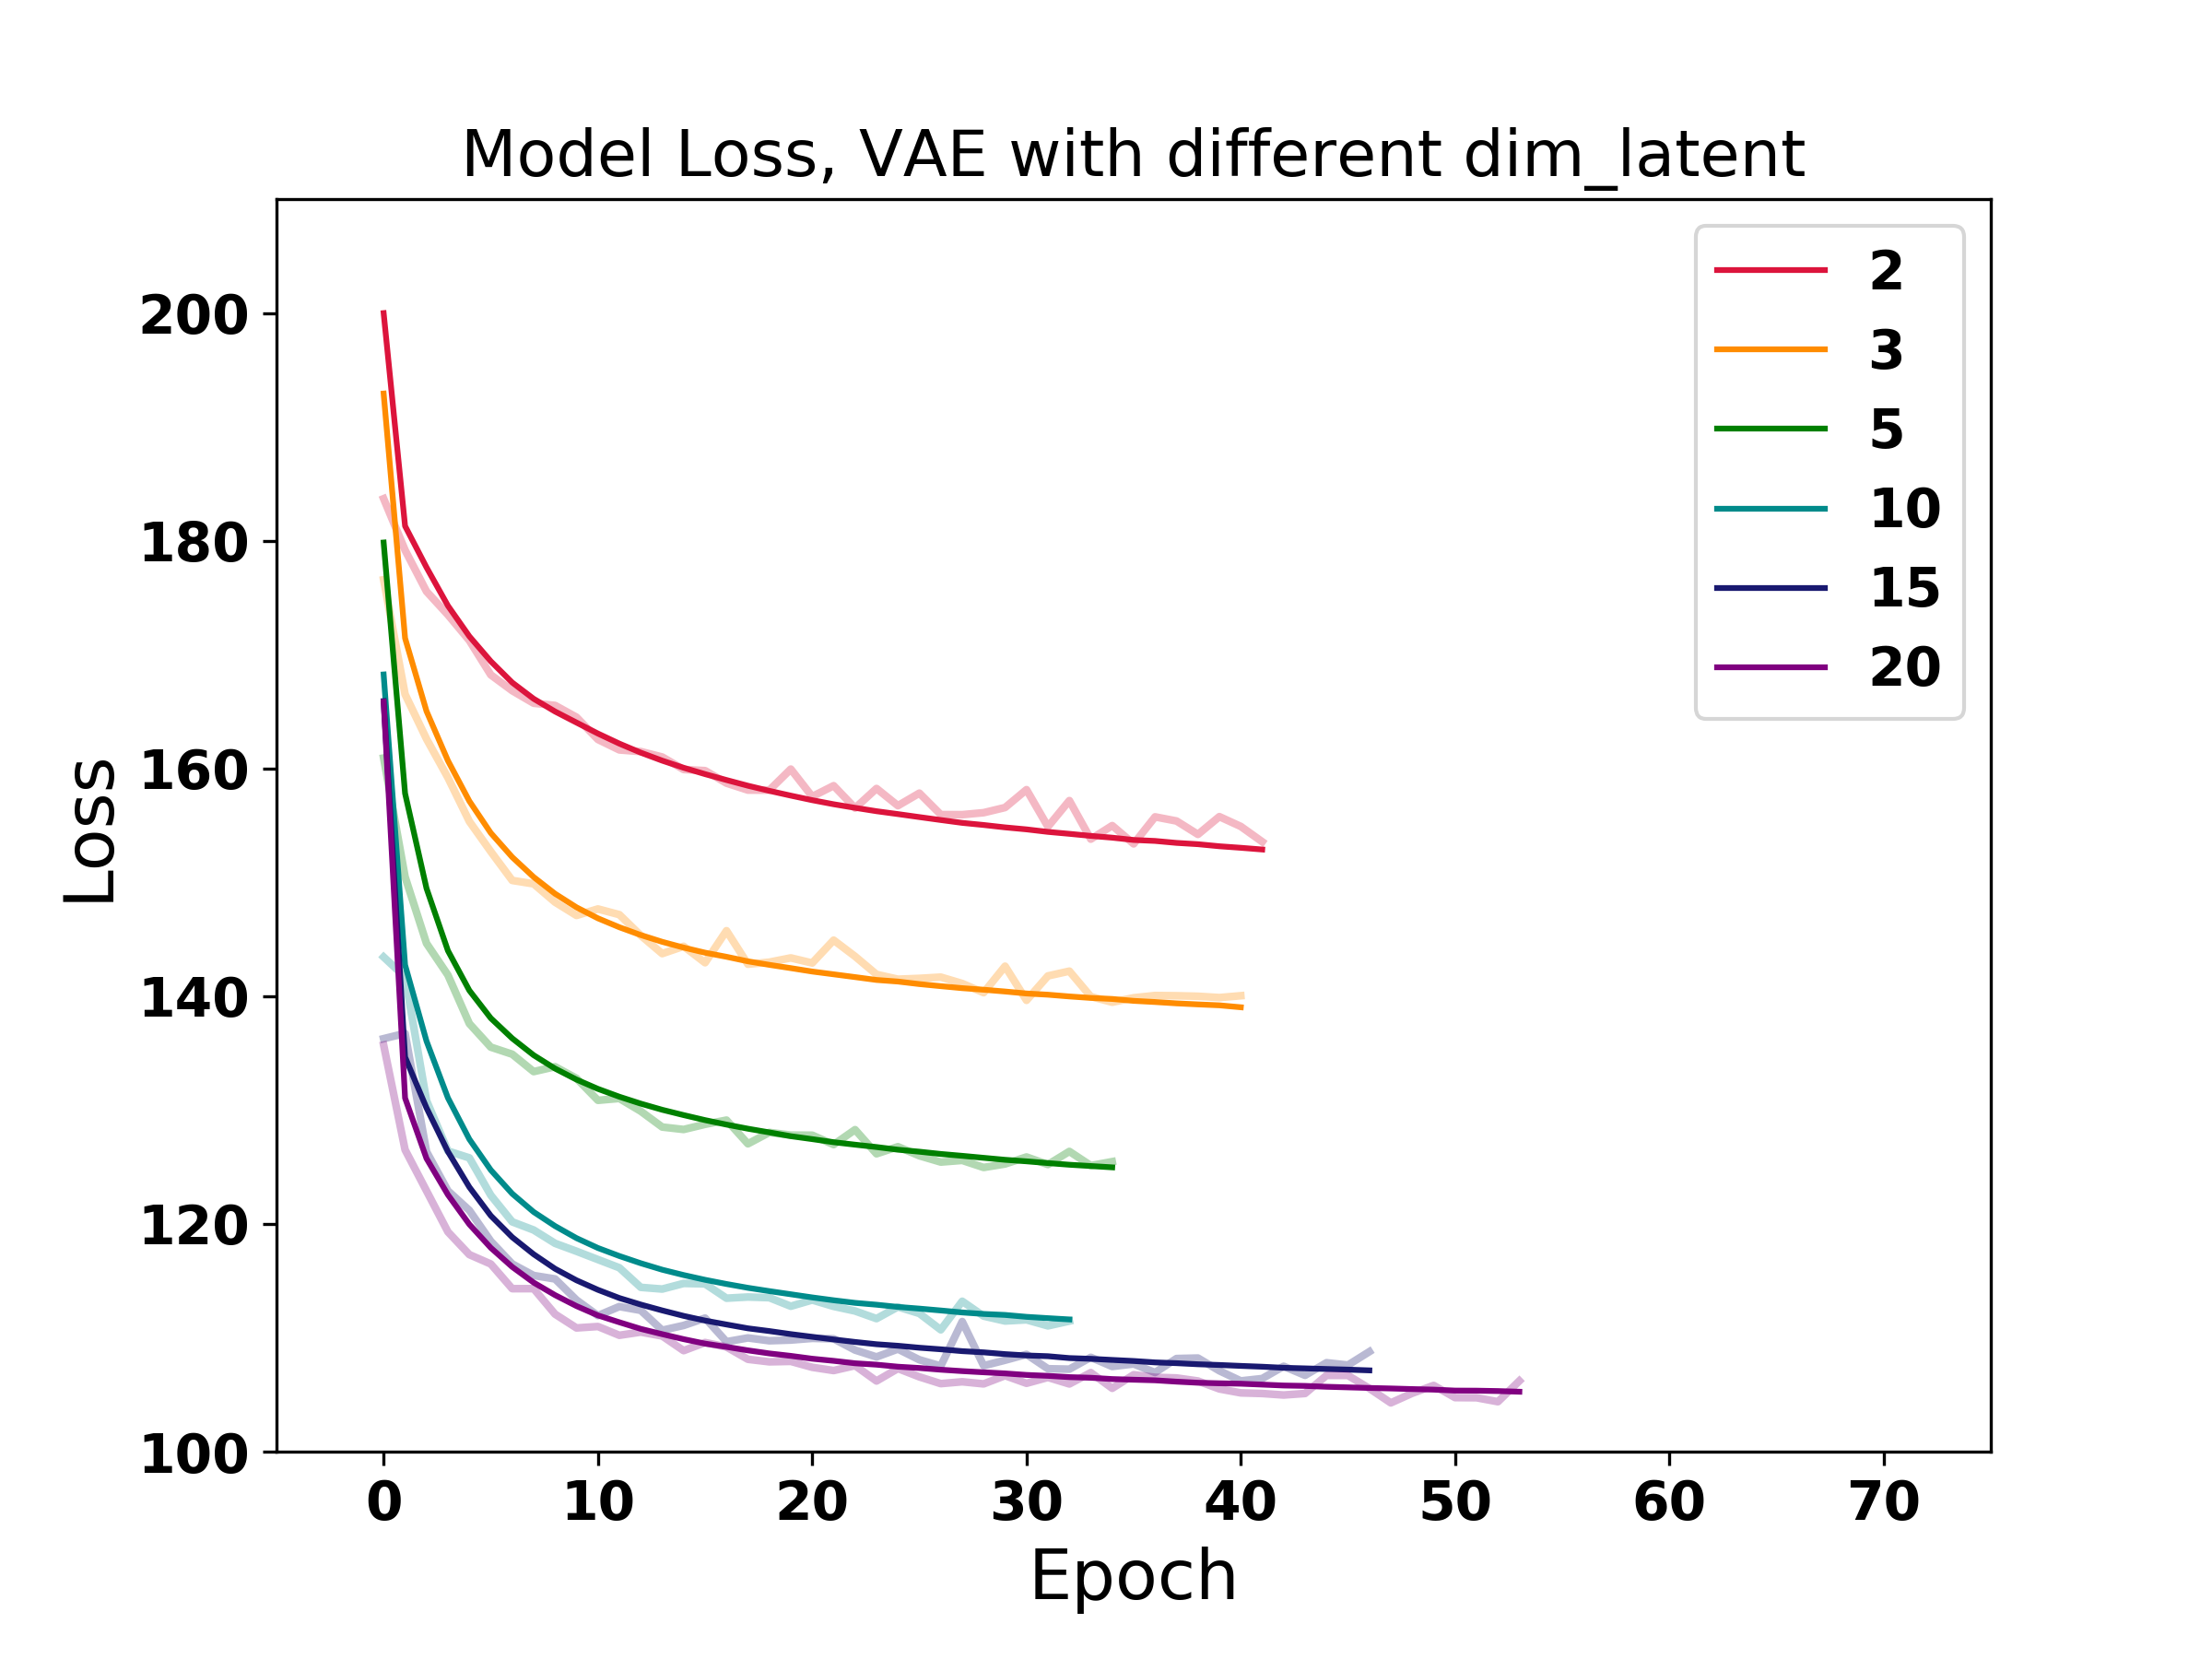
\includegraphics[width=0.47\columnwidth]{fig/latent_exps_early_stop_5.png}
}
\subfigure[over 70 epochs]{\label{fig:b}
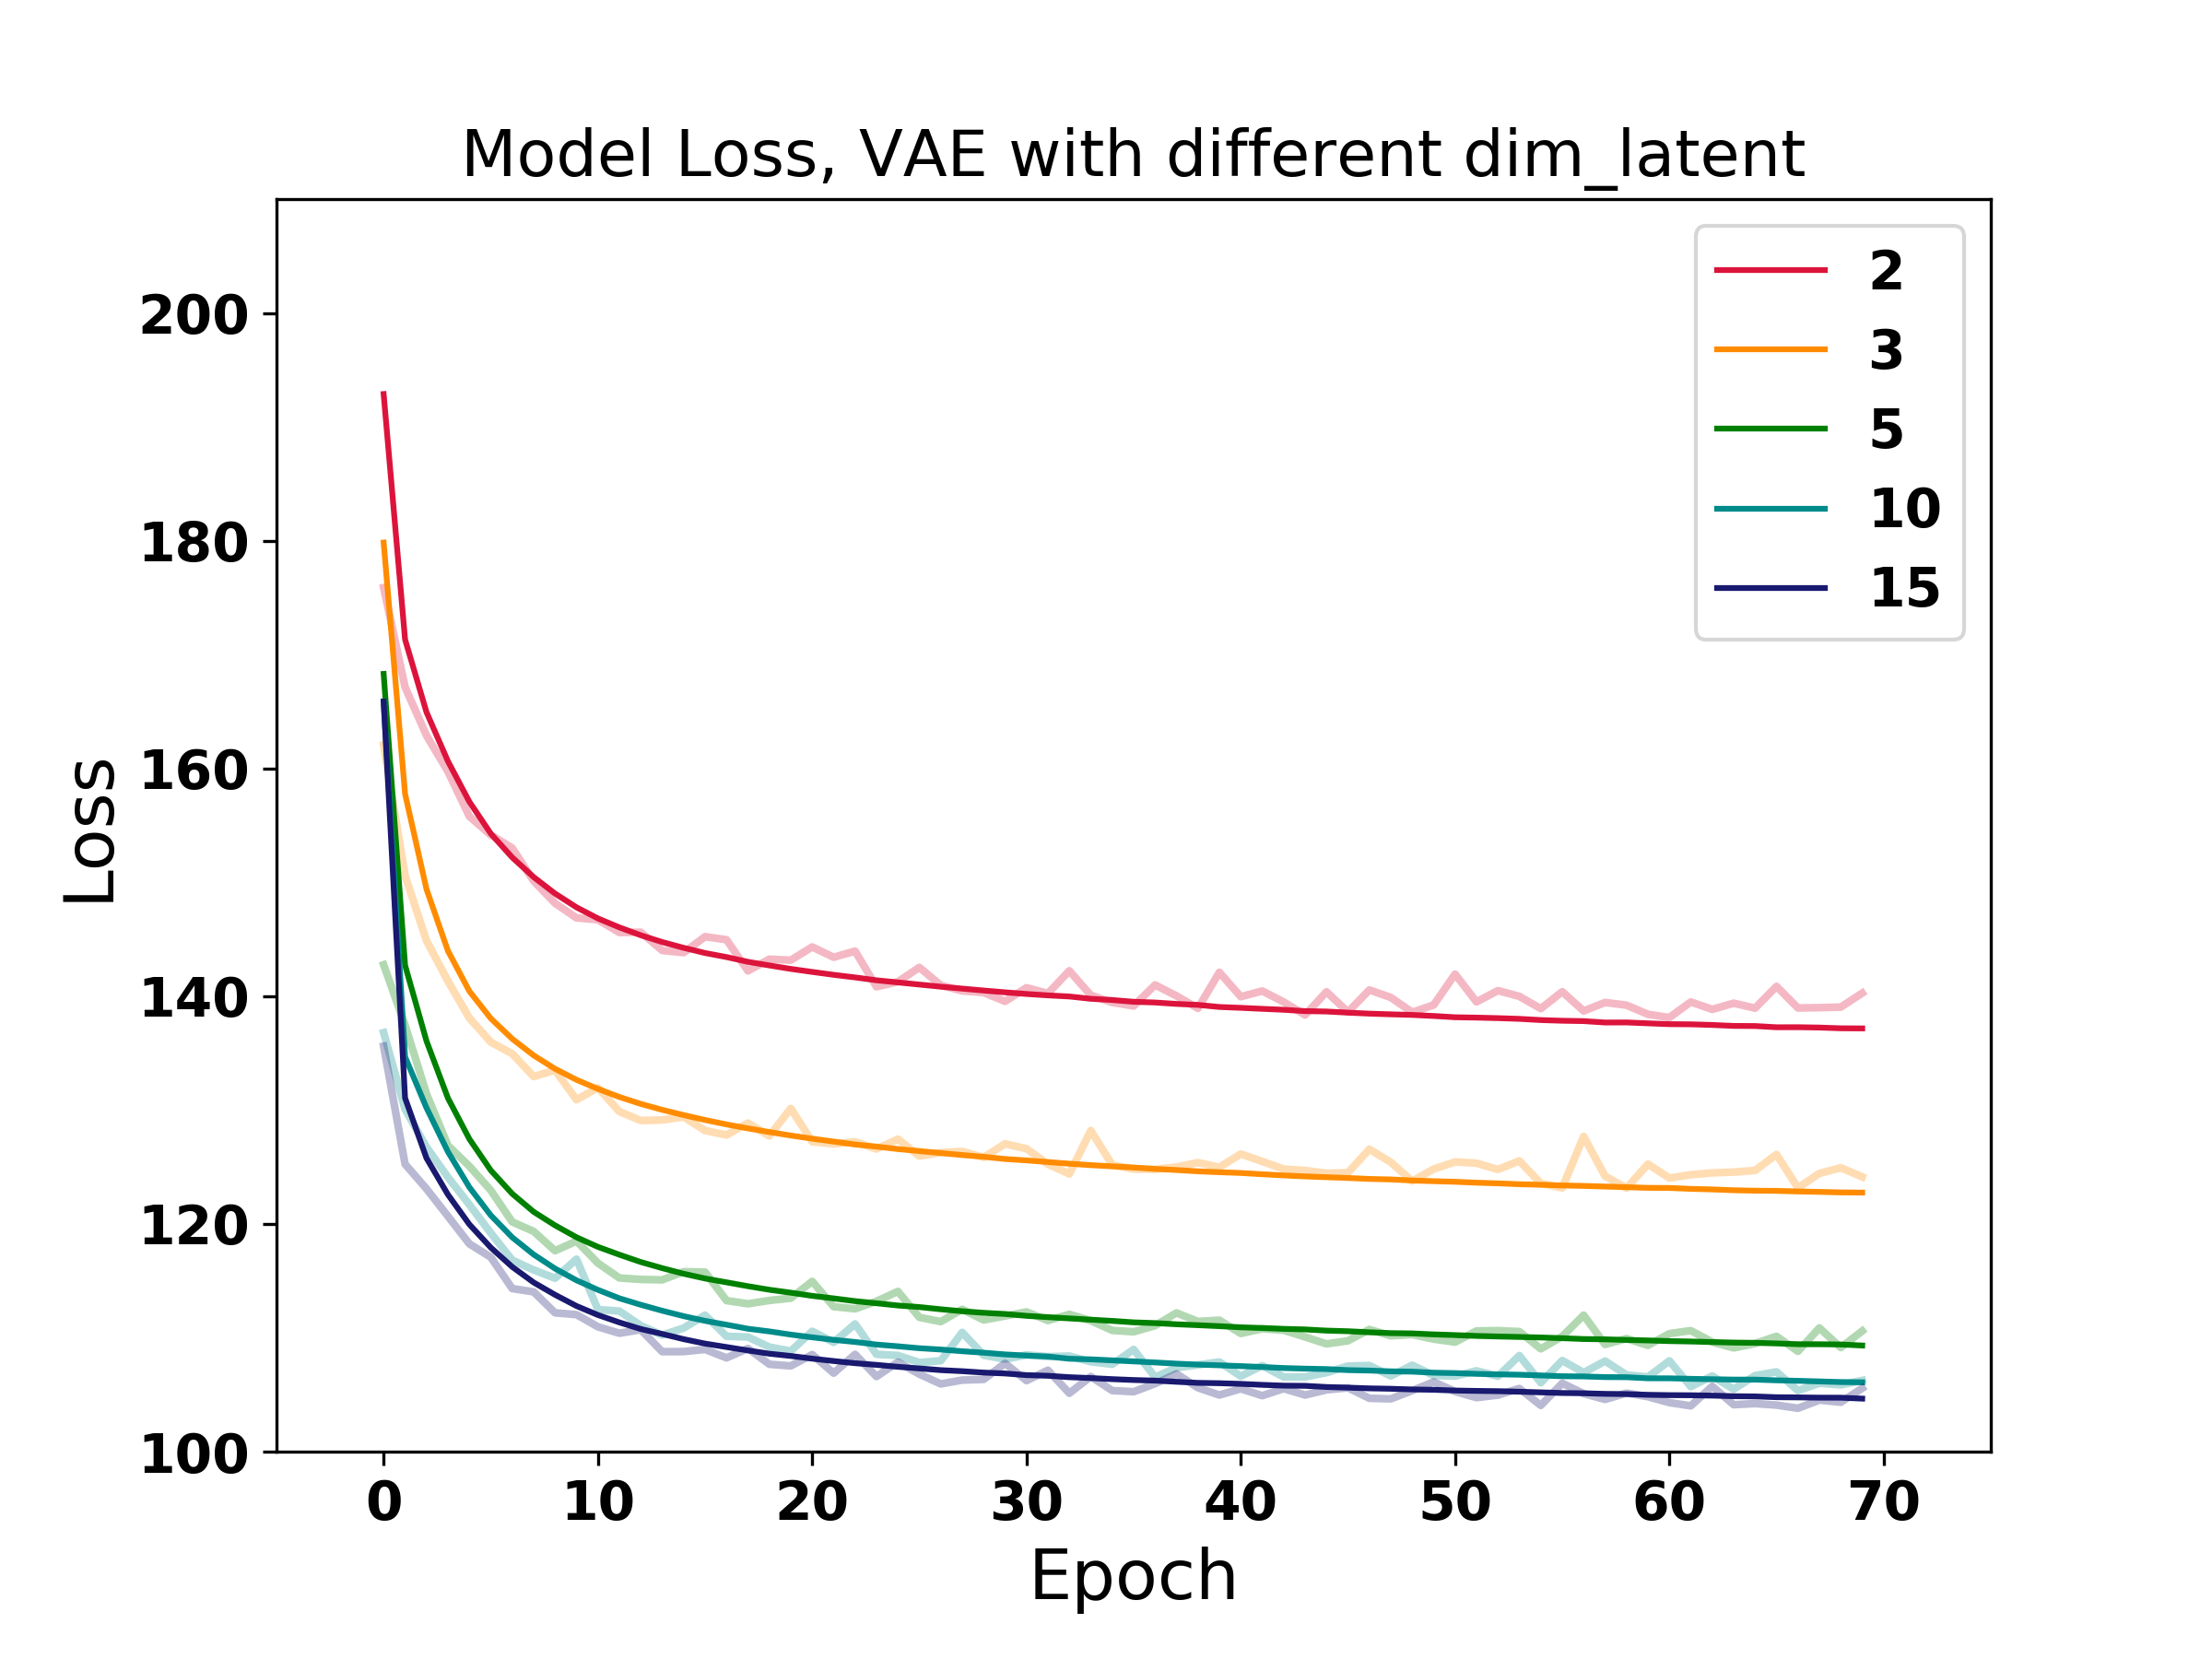
\includegraphics[width=0.47\columnwidth]{fig/latent_exps.png}
}
\caption{Dim Latent = 2,3,5,10,15,20}
\textcolor[RGB]{185 181 205}{\scriptsize 
code: \url{https://github.com/ThitherShore/VAE-toy/blob/master/exps\_diff\_latent.py}\\
patience: number of epochs with no improvement after which training will be stopped.}
\end{figure}
\end{frame}
%%%%%%%%%%%%%%%%%%%%%%%%%%%%%%%%%%%%%%%%%%%%%%%%%%%%%%%%%%%%%
{%BACKGROUND START
\usebackgroundtemplate{
\includegraphics[width=\paperwidth]{fig/BG.png}}
\begin{frame}
\begin{center}
{\bf\LARGE Conditional Variational Auto-Encoder}
\end{center}
\end{frame}
}%BACKGROUND E N D
%%%%%%%%%%%%%%%%%%%%%%%%%%%%%%%%%%%%%%%%%%%%%%%%%%%%%%%%%%%%%
\begin{frame}{Conditional Variational Auto-Encoder (CVAE)}
\begin{figure}
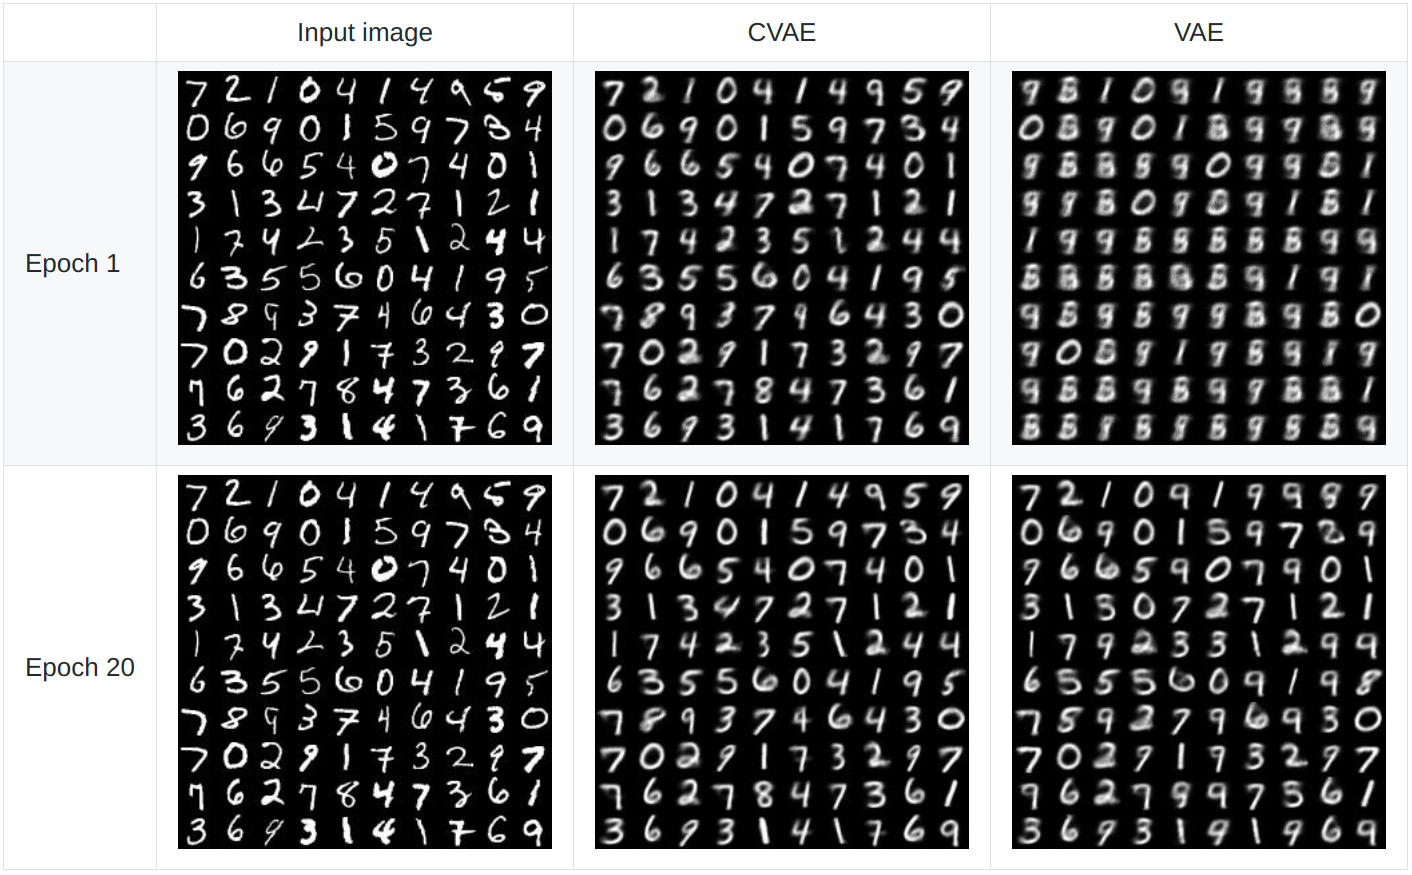
\includegraphics[width=.9\columnwidth]{fig/vs_vae.png}
\begin{spacing}{1}
\textcolor[RGB]{185 181 205}{\small
Ref (paper): \citet[Semi-S L with Deep Generative Models]{kingma5298semi}\\
Ref (codes): \url{https://zhuanlan.zhihu.com/p/25401928}
}
\end{spacing}
\end{figure}
\end{frame}
%%%%%%%%%%%%%%%%%%%%%%%%%%%%%%%%%%%%%%%%%%%%%%%%%%%%%%%%%%%%%
\begin{frame}{Conditional Variational Auto-Encoder (CVAE)}
\begin{figure}
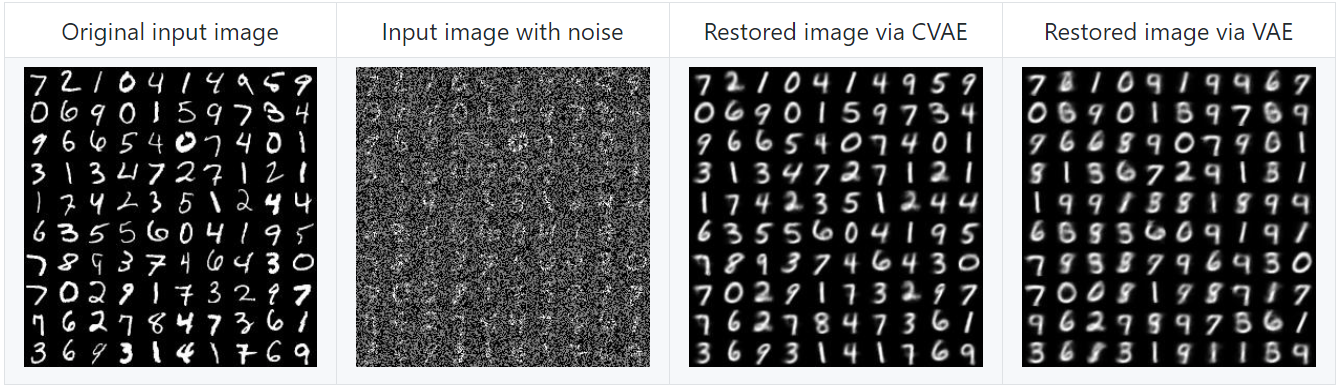
\includegraphics[width=.95\columnwidth]{fig/cvae_recon.png}
\begin{spacing}{1}
\textcolor[RGB]{185 181 205}{\small
Ref: \url{https://zhuanlan.zhihu.com/p/25401928}}
\end{spacing}
\end{figure}
\end{frame}
%%%%%%%%%%%%%%%%%%%%%%%%%%%%%%%%%%%%%%%%%%%%%%%%%%%%%%%%%%%%%
\begin{frame}{Conditional Variational Auto-Encoder (CVAE)}
\begin{figure}
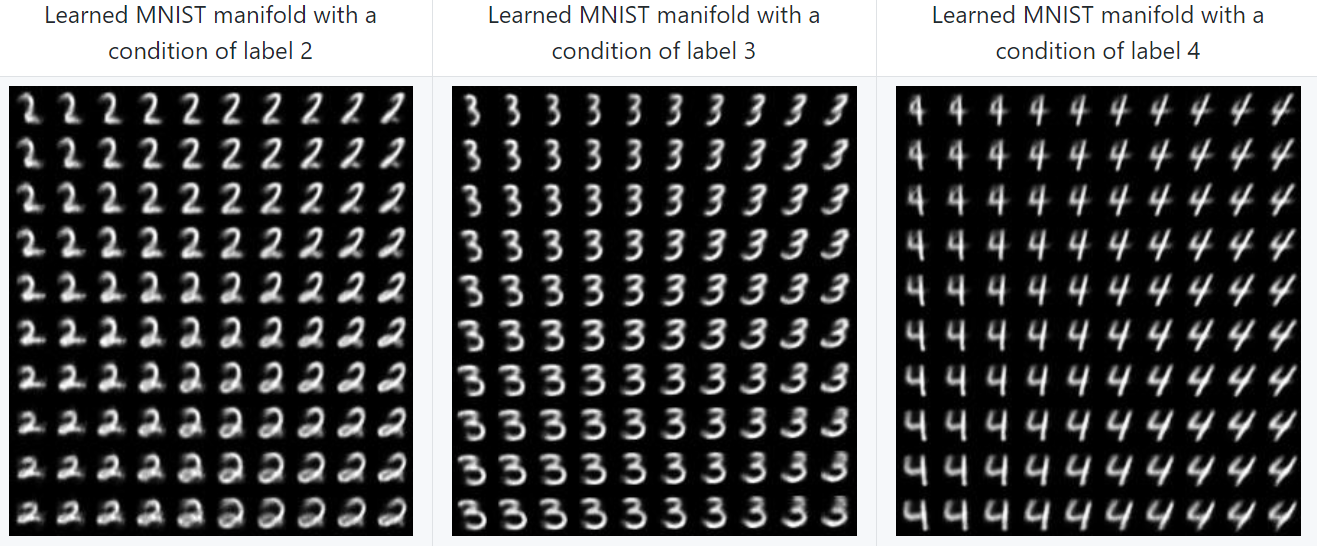
\includegraphics[width=.9\columnwidth]{fig/cvae_condi.png}
\begin{spacing}{1}
\textcolor[RGB]{185 181 205}{\small
Ref: \url{https://zhuanlan.zhihu.com/p/25401928}}
\end{spacing}
\end{figure}
\end{frame}
%%%%%%%%%%%%%%%%%%%%%%%%%%%%%%%%%%%%%%%%%%%%%%%%%%%%%%%%%%%%%
\begin{frame}
\bibliographystyle{abbrvnat}
\bibliography{ref}
\end{frame}
%%%%%%%%%%%%%%%%%%%%%%%%%%%%%%%%%%%%%%%%%%%%%%%%%%%%%%%%%%%%%
\begin{frame}
\begin{center}
{\LARGE Thank You!}
\end{center}
\end{frame}
%%%%%%%%%%%%%%%%%%%%%%%%%%%%%%%%%%%%%%%%%%%%%%%%%%%%%%%%%%%%%
\end{document}
